% ******************************* PhD Thesis Template **************************
% Please have a look at the README.md file for info on how to use the template

\documentclass[a4paper,12pt,twoside,numbered,index,custommargin]{Classes/PhDThesisPSnPDF}

% ******************************************************************************
% ******************************* Class Options ********************************
% *********************** See README for more details **************************
% ******************************************************************************

% `a4paper'(The University of Cambridge PhD thesis guidelines recommends a page
% size a4 - default option) or `a5paper': A5 Paper size is also allowed as per
% the Cambridge University Engineering Deparment guidelines for PhD thesis
%
% `11pt' or `12pt'(default): Font Size 10pt is NOT recommended by the University
% guidelines
%
% `oneside' or `twoside'(default): Printing double side (twoside) or single
% side.
%
% `print': Use `print' for print version with appropriate margins and page
% layout. Leaving the options field blank will activate Online version.
%
% `index': For index at the end of the thesis
%
% `draftclassic': For draft mode without loading any images (same as draft in book)
%
% `draft': Special draft mode with line numbers, images, and water mark with
% timestamp and custom text. Position of the text can also be modified.
%
% `abstract': To generate only the title page and abstract page with
% dissertation title and name, to submit to the Student Registry
%
% `chapter`: This option enables only the specified chapter and it's references
%  Useful for review and corrections.
%
% ************************* Custom Page Margins ********************************
%
% `custommargin`: Use `custommargin' in options to activate custom page margins,
% which can be defined in the preamble.tex. Custom margin will override
% print/online margin setup.
%
% *********************** Choosing the Fonts in Class Options ******************
%
% `times' : Times font with math support. (The Cambridge University guidelines
% recommend using times)
%
% `fourier': Utopia Font with Fourier Math font (Font has to be installed)
%            It's a free font.
%
% `customfont': Use `customfont' option in the document class and load the
% package in the preamble.tex
%
% default or leave empty: `Latin Modern' font will be loaded.
%
% ********************** Choosing the Bibliography style ***********************
%
% `authoryear': For author-year citation eg., Krishna (2013)
%
% `numbered': (Default Option) For numbered and sorted citation e.g., [1,5,2]
%
% `custombib': Define your own bibliography style in the `preamble.tex' file.
%              `\RequirePackage[square, sort, numbers, authoryear]{natbib}'.
%              This can be also used to load biblatex instead of natbib
%              (See Preamble)
%
% **************************** Choosing the Page Style *************************
%
% `default (leave empty)': For Page Numbers in Header (Left Even, Right Odd) and
% Chapter Name in Header (Right Even) and Section Name (Left Odd). Blank Footer.
%
% `PageStyleI': Chapter Name next & Page Number on Even Side (Left Even).
% Section Name & Page Number in Header on Odd Side (Right Odd). Footer is empty.
%
% `PageStyleII': Chapter Name on Even Side (Left Even) in Header. Section Number
% and Section Name in Header on Odd Side (Right Odd). Page numbering in footer

% Uncomment to change page style
%\pagestyle{PageStyleII}

% ********************************** Preamble **********************************
% Preamble: Contains packages and user-defined commands and settings
% ******************************************************************************
% ****************************** Custom Margin *********************************

% Add `custommargin' in the document class options to use this section
% Set {innerside margin / outerside margin / topmargin / bottom margin}  and
% other page dimensions
\ifsetCustomMargin
  \RequirePackage[left=25mm,right=25mm,top=35mm,bottom=30mm, bindingoffset = 0.5in]{geometry}
  \setFancyHdr % To apply fancy header after geometry package is loaded
\fi

% Add spaces between paragraphs
%\setlength{\parskip}{0.5em}
% Ragged bottom avoids extra whitespaces between paragraphs
\raggedbottom
% To remove the excess top spacing for enumeration, list and description
%\usepackage{enumitem}
%\setlist[enumerate,itemize,description]{topsep=0em}

% *****************************************************************************
% ******************* Fonts (like different typewriter fonts etc.)*************

% Add `customfont' in the document class option to use this section

\ifsetCustomFont
  % Set your custom font here and use `customfont' in options. Leave empty to
  % load computer modern font (default LaTeX font).
  %\RequirePackage{helvet}

  % For use with XeLaTeX
  %  \setmainfont[
  %    Path              = ./libertine/opentype/,
  %    Extension         = .otf,
  %    UprightFont = LinLibertine_R,
  %    BoldFont = LinLibertine_RZ, % Linux Libertine O Regular Semibold
  %    ItalicFont = LinLibertine_RI,
  %    BoldItalicFont = LinLibertine_RZI, % Linux Libertine O Regular Semibold Italic
  %  ]
  %  {libertine}
  %  % load font from system font
  %  \newfontfamily\libertinesystemfont{Linux Libertine O}
\fi

% *****************************************************************************
% **************************** Custom Packages ********************************

% ************************* Algorithms and Pseudocode **************************

%\usepackage{algpseudocode}


% ********************Captions and Hyperreferencing / URL **********************

% Captions: This makes captions of figures use a boldfaced small font.
%\RequirePackage[small,bf]{caption}

\RequirePackage[labelsep=space,tableposition=top]{caption}
\renewcommand{\figurename}{Fig.} %to support older versions of captions.sty


% *************************** Graphics and figures *****************************

%\usepackage{rotating}
%\usepackage{wrapfig}

% Uncomment the following two lines to force Latex to place the figure.
% Use [H] when including graphics. Note 'H' instead of 'h'
%\usepackage{float}
%\restylefloat{figure}

% Subcaption package is also available in the sty folder you can use that by
% uncommenting the following line
% This is for people stuck with older versions of texlive
%\usepackage{sty/caption/subcaption}
\usepackage{subcaption}
\usepackage{tikz}
\usepackage[ruled,vlined]{algorithm2e}
\usepackage{amsmath}
\usepackage{amssymb}
\usepackage{amsthm}

% ********************************** Tables ************************************
\usepackage{booktabs} % For professional looking tables
\usepackage{multirow}

%\usepackage{multicol}
%\usepackage{longtable}
%\usepackage{tabularx}


% *********************************** SI Units *********************************
\usepackage{siunitx} % use this package module for SI units


% ******************************* Line Spacing *********************************

% Choose linespacing as appropriate. Default is one-half line spacing as per the
% University guidelines

% \doublespacing
\onehalfspacing
% \singlespacing


% ************************ Formatting / Footnote *******************************

% Don't break enumeration (etc.) across pages in an ugly manner (default 10000)
%\clubpenalty=500
%\widowpenalty=500

%\usepackage[perpage]{footmisc} %Range of footnote options


% *****************************************************************************
% *************************** Bibliography  and References ********************

%\usepackage{cleveref} %Referencing without need to explicitly state fig /table

% Add `custombib' in the document class option to use this section
\ifuseCustomBib
   \RequirePackage[square, sort, numbers, authoryear]{natbib} % CustomBib

% If you would like to use biblatex for your reference management, as opposed to the default `natbibpackage` pass the option `custombib` in the document class. Comment out the previous line to make sure you don't load the natbib package. Uncomment the following lines and specify the location of references.bib file

%\RequirePackage[backend=biber, style=numeric-comp, citestyle=numeric, sorting=nty, natbib=true]{biblatex}
%\bibliography{References/references} %Location of references.bib only for biblatex

\fi

% changes the default name `Bibliography` -> `References'
\renewcommand{\bibname}{References}


% ******************************************************************************
% ************************* User Defined Commands ******************************
% ******************************************************************************

% *********** To change the name of Table of Contents / LOF and LOT ************

%\renewcommand{\contentsname}{My Table of Contents}
%\renewcommand{\listfigurename}{My List of Figures}
%\renewcommand{\listtablename}{My List of Tables}


% ********************** TOC depth and numbering depth *************************

\setcounter{secnumdepth}{2}
\setcounter{tocdepth}{2}


% ******************************* Nomenclature *********************************

% To change the name of the Nomenclature section, uncomment the following line

%\renewcommand{\nomname}{Symbols}


% ********************************* Appendix ***********************************

% The default value of both \appendixtocname and \appendixpagename is `Appendices'. These names can all be changed via:

%\renewcommand{\appendixtocname}{List of appendices}
%\renewcommand{\appendixname}{Appndx}

% *********************** Configure Draft Mode **********************************

% Uncomment to disable figures in `draft'
%\setkeys{Gin}{draft=true}  % set draft to false to enable figures in `draft'

% These options are active only during the draft mode
% Default text is "Draft"
%\SetDraftText{DRAFT}

% Default Watermark location is top. Location (top/bottom)
%\SetDraftWMPosition{bottom}

% Draft Version - default is v1.0
%\SetDraftVersion{v1.1}

% Draft Text grayscale value (should be between 0-black and 1-white)
% Default value is 0.75
%\SetDraftGrayScale{0.8}


% ******************************** Todo Notes **********************************
%% Uncomment the following lines to have todonotes.

%\ifsetDraft
%	\usepackage[colorinlistoftodos]{todonotes}
%	\newcommand{\mynote}[1]{\todo[author=kks32,size=\small,inline,color=green!40]{#1}}
%\else
%	\newcommand{\mynote}[1]{}
%	\newcommand{\listoftodos}{}
%\fi

% Example todo: \mynote{Hey! I have a note}
\newtheorem{theorem}{Theorem}[section]
\newtheorem{lemma}[theorem]{Lemma}
\newtheorem{proposition}[theorem]{Proposition}
\newtheorem{corollary}[theorem]{Corollary}

\newenvironment{definition}[1][Definition]{\begin{trivlist}
\item[\hskip \labelsep {\bfseries #1}]}{\end{trivlist}}
\newenvironment{example}[1][Example]{\begin{trivlist}
\item[\hskip \labelsep {\bfseries #1}]}{\end{trivlist}}
\newenvironment{remark}[1][Remark]{\begin{trivlist}
\item[\hskip \labelsep {\bfseries #1}]}{\end{trivlist}}

% ************************ Thesis Information & Meta-data **********************
% Thesis title and author information, refernce file for biblatex
% ************************ Thesis Information & Meta-data **********************
%% The title of the thesis
\title{Scaling Behaviour of SAT: Theory and Practice}
%\texorpdfstring is used for PDF metadata. Usage:
%\texorpdfstring{LaTeX_Version}{PDF Version (non-latex)} eg.,
%\texorpdfstring{$sigma$}{sigma}

%% Subtitle (Optional)
\subtitle{An exposition on the gap between theoretical conditional lower bounds for SAT and the practical performance of SAT solvers}

%% The full name of the author
\author{Eavan Thomas Pattie}

%% Department (eg. Department of Engineering, Maths, Physics)
\dept{Department of Computer Science}

%% University and Crest
\university{University of Warwick}
% Crest minimum should be 30mm.
\crest{
\includegraphics[width=0.2\textwidth]{crest.png}}
%% Use this crest, if you are using the college crest
%% Crest long miminum should be 65mm
%\crest{
\includegraphics[width=0.45\textwidth]{University_Crest_Long}}

%% College shield [optional] 
% Crest minimum should be 30mm.
%\collegeshield{
\includegraphics[width=0.2\textwidth]{CollegeShields/Kings}}


%% Supervisor (optional)
%% for multiple supervisors, append each supervisor with the \newline command
\supervisor{Dmitry Chistikov}
%Prof. C.D. Supervisor}

%% Supervisor Role (optional) - Supervisor (default) or advisor
% \supervisorrole{\textbf{Supervisors: }}
%% if no title is desired:
% \supervisorrole{}

%% Supervisor line width: required to align supervisors
%\supervisorlinewidth{0.35\textwidth}

%% Advisor (optional)
%% for multiple advisors, append each advisor with the \newline command
%\advisor{Dr. A. Advisor\newline
%Dr. B. Advisor}
     
%% Advisor Role (optional) - Advisor (default) or leave empty
% \advisorrole{Advisors: }
%% if no title is required
% \advisorrole{}

%% Advisor line width: required to align supervisors
%\advisorlinewidth{0.25\textwidth}


%% You can redefine the submission text:
% Default as per the University guidelines:
% ``This dissertation is submitted for the degree of''
\renewcommand{\submissiontext}{Year of Study: 3rd}

%% Full title of the Degree
%\degreetitle{Masters of Engineering}

%% Submission date
% Default is set as {\monthname[\the\month]\space\the\year}
%\degreedate{September 2014} 

%% Meta information
\subject{Boolean Satisfiability Problem} \keywords{{SAT} {3rd Year Project}}


% ***************************** Abstract Separate ******************************
% To printout only the titlepage and the abstract with the PhD title and the
% author name for submission to the Student Registry, use the `abstract' option in
% the document class.

\ifdefineAbstract
 \pagestyle{empty}
 \includeonly{Declaration/declaration, Abstract/abstract}
\fi

% ***************************** Chapter Mode ***********************************
% The chapter mode allows user to only print particular chapters with references
% Title, Contents, Frontmatter are disabled by default
% Useful option to review a particular chapter or to send it to supervisior.
% To use choose `chapter' option in the document class

\ifdefineChapter
 \includeonly{Chapter3/chapter3}
\fi

% ******************************** Front Matter ********************************
\begin{document}

\frontmatter

\maketitle

%% ******************************* Thesis Dedidcation ********************************

\begin{dedication} 

I would like to dedicate this thesis to my loving parents \dots

\end{dedication}
%% ******************************* Thesis Declaration ***************************

\begin{declaration}

I hereby declare that except where specific reference is made to the work of 
others, the contents of this dissertation are original and have not been 
submitted in whole or in part for consideration for any other degree or 
qualification in this, or any other university. This dissertation is my own 
work and contains nothing which is the outcome of work done in collaboration 
with others, except as specified in the text and Acknowledgements. This 
dissertation contains fewer than 65,000 words including appendices, 
bibliography, footnotes, tables and equations and has fewer than 150 figures.

% Author and date will be inserted automatically from thesis.tex \author \degreedate

\end{declaration}
% ************************** Thesis Acknowledgements **************************

\begin{acknowledgements}      

I would like acknowledge my supervisor Dmitry Chistikov for our valuable conversations
and guidance, without which the project would not have been completed.
I would also like to thank Gabriel\.e Stravinskait\.e for her continued
support throughout the project. I'd like to thank my family
for keeping my progress in check, and finally I would like to thank
Ava, Aaron, Nicola and Michal for their help with typesetting and general
support.

\end{acknowledgements}

% ************************** Thesis Abstract *****************************
% Use `abstract' as an option in the document class to print only the titlepage and the abstract.
\begin{abstract}
The Boolean Satisfiability Problem (SAT) is a well studied NP-COMPLETE
problem for which there exists no known algorithm faster than 
$\mathcal{O}^{\ast}(2^n)$
where $n$ is the number of variables. However, fast ``in practice'' SAT solvers
have been developed that are used in a wide range of domains. We give an
introduction into how these solvers function and contrast their performance with the
conditional lower bounds that can be shown via hypotheses about the complexity
of SAT. We detail the sparsification lemma, a critical technique used to show these
lower bounds. Finally, we cover observations about the structure of SAT that
modern solvers exploit to achieve speeds faster than what worst case complexity
would suggest.

\emph{Keywords}: SAT, SAT Solvers, Conditional Lower Bounds, Subexponential Time, Phase Transition, Backdoor sets, Sparsification Lemma
\end{abstract}


% *********************** Adding TOC and List of Figures ***********************

\tableofcontents

\listoffigures

\listoftables

% \printnomenclature[space] space can be set as 2em between symbol and description
%\printnomenclature[3em]

\printnomenclature

% ******************************** Main Matter *********************************
\mainmatter

%!TEX root = ../thesis.tex
%*******************************************************************************
%*********************************** First Chapter *****************************
%*******************************************************************************

\chapter{Introduction}  %Title of the First Chapter

\ifpdf
    \graphicspath{{Chapter1/Figs/Raster/}{Chapter1/Figs/PDF/}{Chapter1/Figs/}}
\else
    \graphicspath{{Chapter1/Figs/Vector/}{Chapter1/Figs/}}
\fi


%**********************************

%********************************** %First Section  **************************************

\nomenclature[x]{$F$}{Boolean Formula}
\nomenclature[z-CNF]{CNF}{Conjunctive Normal Form}
\nomenclature[z-DNF]{DNF}{Disjunctive Normal Form}
\nomenclature[z-SAT]{SAT}{Boolean Satisfiability Problem}
\nomenclature[z-kSAT]{$k$-SAT}{Boolean Satisfiability Problem with each clause
                               restricted to have size $k$ or less}

\begin{figure}
    \centering
    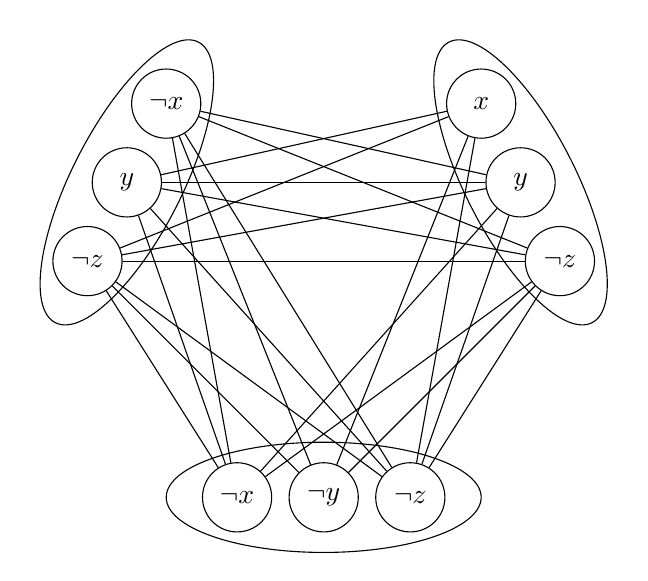
\begin{tikzpicture}
        \begin{scope}[auto,every node/.style={draw,circle,minimum size=2.5em}]
            % Clause 1
            \node (c1!x) at (-2, 0) {$\neg x$};
            \node (c1y) at (-2.5, -1) {$y$};
            \node (c1!z) at (-3, -2) {$\neg z$};
            \draw[rotate around={63:(-2.5,-1)}] (-2.5,-1) ellipse (2 and 0.7);

            % Clause 2
            \node (c2x) at (2, 0) {$x$};
            \node (c2y) at (2.5, -1) {$y$};
            \node (c2!z) at (3, -2) {$\neg z$};
            \draw[rotate around={-63:(2.5,-1)}] (2.5,-1) ellipse (2 and 0.7);

            % Clause 2
            \node (c3!x) at (-1.1, -5) {$\neg x$};
            \node (c3!y) at (0, -5) {$\neg y$};
            \node (c3!z) at (1.1, -5) {$\neg z$};
            \draw[] (0,-5) ellipse (2 and 0.7);
        \end{scope}
        
        \path (c1!x) edge (c2y);
        \path (c1!x) edge (c2!z);
        \path (c1!x) edge (c3!x);
        \path (c1!x) edge (c3!y);
        \path (c1!x) edge (c3!z);
        \path (c1y) edge (c2x);
        \path (c1y) edge (c2y);
        \path (c1y) edge (c2!z);
        \path (c1y) edge (c3!x);
        \path (c1y) edge (c3!z);
        \path (c1!z) edge (c2x);
        \path (c1!z) edge (c2y);
        \path (c1!z) edge (c2!z);
        \path (c1!z) edge (c3!x);
        \path (c1!z) edge (c3!y);
        \path (c1!z) edge (c3!z);
        
        \path (c2x) edge (c3!y);
        \path (c2x) edge (c3!z);
        \path (c2y) edge (c3!x);
        \path (c2y) edge (c3!z);
        \path (c2!z) edge (c3!x);
        \path (c2!z) edge (c3!y);
        \path (c2!z) edge (c3!z);
    \end{tikzpicture}
    \caption[Graph Representation of a 3SAT Formula]{Illustration of the 3SAT in Equation \ref{eq:formula_sat}. Vertices are grouped
    by their clauses and the edges
    represent literals that do not contradict. This establishes a reduction
    from 3SAT to clique}
    \label{fig:sat}
\end{figure}

\section{Boolean Satisfiability Problem} %Section - 1.1 
The boolean satisfiability problem, abbreviated as SAT, is the problem of finding
a satisfying assignment to the variables to make a boolean formula evaluate to true.
CNF-SAT is the same problem, but with formulas restricted to Conjunctive Normal Form
(CNF). A boolean formula in CNF is composed of a conjunction of clauses where
each clause is a disjunction of literals. For example consider the following
boolean formula in CNF: 
\begin{equation} \label{eq:formula_sat}
    (\neg x \lor y \lor \neg z) \land (x \lor y \lor \neg z) \land (\neg x \lor \neg y \lor \neg z)
\end{equation}
This boolean formula has
a satisfying assignment $x = \text{false}, y = \text{true}, z = \text{false}$. Therefore the boolean formula is satisfiable.
However, if we consider the boolean formula
\begin{align}
(x \lor y \lor z)\land(x \lor y \lor \neg z)\land(x \lor \neg y \lor z) \nonumber\\
\land(x \lor \neg y \lor \neg z)\land(\neg x \lor y \lor z)\land(\neg x \lor y \lor \neg z) \\
\land(\neg x \lor \neg y \lor z)\land(\neg x \lor \neg y \lor \neg z) \nonumber
\end{align}
It's clear to see that this boolean formula can have no
satisfying assignment, since each assignment to the variables
will at least leave one clause unsatisfied.

%********************************** %Second Section  *************************************
\section{Uses of Boolean Satisfiability} %Section - 1.2
\subsection{Theoretical Significance}
SAT is a widely studied problem and has had a significant impact on
our understanding of computational complexity. For instance, SAT
was the first problem shown to be NP-HARD.
This then forms the basis of the NP-COMPLETE complexity class \cite{cook1971complexity, karp1972reducibility}.
This then means that a large class of problems all can be reduced to each other \cite{garey1974some}.
SAT has then in some sense become the defacto NP-COMPLETE problem and
our understanding of NP-COMPLETEness is driven by our understanding of SAT.

Furthermore, study of SAT has lead to new conjectures about
the complexity of SAT that are stronger than
the $P \neq NP$ conjecture, roughly stating that SAT requires exponential time \cite{impagliazzo2001complexity}. These conjectures allow for new conditional lower
bounds on a wide variety of other problems, not strictly limited to
NP-COMPLETE problems \cite{vassilevska2015hardness, lokshtanov2013lower}.
This gives us an understanding of the relative difficulty of finding
improved algorithms for many computational problems. For instance,
we know that finding a $\mathcal{O}(n^{2 - \epsilon})$ time algorithm
for string edit distance would violate some of these conjectures \cite{vassilevska2015hardness, levenshtein1966binary}. Hence making an improvement over an $\mathcal{O}(n^2)$ algorithm
should be seen as being as hard as discovering an improved SAT algorithm.

\subsection[Practical Applications]{Practical Applications of Boolean Satisfiability}
Although, even with these conjectures about the hardness of SAT,
as SAT solvers have become more efficient, SAT solving has found numerous applications \cite{marques2008practical, sat2009theory}.
One of these applications is model checking, where
the use SAT allows for better memory usage than traditional methods and hence larger models \cite{biere1999symbolic}.
Others include, but are not limited to, crosstalk noise prediction in integrated circuits \cite{chen1999towards},
termination analysis \cite{fuhs2007sat}, design debugging \cite{smith2005fault}, AI planning \cite{kautz1992planning},
haplotype  inference  in  bioinformatics \cite{lynce2006efficient}, knowledge-compilation \cite{darwiche2004new},
software testing \cite{khurshid2004testera}, package management in software distributions \cite{tucker2007opium},
checking of pedigree consistency \cite{10.1007/978-3-540-71209-1_26}, Test-pattern generation in digital systems
\cite{larrabee1992test} and circuit delay computation \cite{mcgeer1991timing}.

Naturally, as the computational power available to SAT solvers grows and as the
solvers become more efficient, SAT solving will find more
practical applications.

%********************************** % Third Section  *************************************
\section{Organisation and Motivation For This Report}  %Section - 1.3 
%NP-COMPLETE decision problems such as SAT and variants such as 3SAT,
%do not have any polynomial time algorithms unless $P=NP$ \cite{schaefer1978complexity}.
%However, SAT is a useful problem in practice \cite{marques2008practical}.
%Therefore, algorithms for solving SAT such as the 
%Davis Putnam Logemann Loveland algorithm (DPLL) and
%Conflict Driven Clause Learning (CDCL) have been developed \cite{Quest_for_efficient_solvers, CDCL}.
%Solvers based on these algorithms appear to be ``fast'' in practice \cite{SAT_Comp2017}.
%At the same time, there are popular conjectures about the complexity
%of SAT that are stronger than assuming $P=NP$ \cite{impagliazzo2001complexity}. These conjectures
%allow theoreticians to prove conditional lower bounds on a wide
%array of problems \cite{lokshtanov2013lower, vassilevska2015hardness}. 
There is a juxtaposition of theory and practice where conjectures about the computational complexity of
SAT suggest that we should not expect it to be solvable in subexponential time \cite{impagliazzo2001complexity},
and yet there are highly optimised SAT solvers that are ``fast'' in practice. Some
of these solvers are able to handle SAT instances having on the order of $10^5$ variables
and $10^6$ clauses \cite{SAT_Comp2017, sat2018descriptions}.
This report will attempt to provide an exposition on this
gap between theory and practice. 

First this will be done by providing an overview of how modern SAT solvers work,
by both covering the algorithms that these solvers are based on and also some
of the implemented solvers that use these algorithms.

To contrast this, the next two chapters will cover the complexity conjectures
that are based on the hardness of SAT and will go over some conditional lower bounds that can be
proven using these conjectures. This report also decides to dedicate a chapter to a commonly used lemma
in these proofs called the sparsification lemma. This lemma is instrumental in many
conditional lower bounds that apply to polynomial time algorithms such as string edit distance, hence
this chapter will explain and go over the proof of the lemma, providing some new intuitions along the way.

Finally, the last chapter will cover some research into structures in SAT instances
that can be used to either explain why some SAT instances are easy to solve compared to what
the worst case complexity of SAT solving would suggest, or provide motivation for currently employed
heuristics in modern SAT solvers.

Taken as a whole this report will provide the reader with a foundational understanding
of both how practical SAT solvers work and how they are able
to solve SAT instances that are significantly larger than what we might expect were possible
given what worst case complexity suggests. This report attempts to be accessible
to anyone with an undergraduate level understanding of computational complexity and algorithms
who is interesting in both the practical and theoretical side of SAT.

%To understand the apparent gap between worst case complexity and practical performance
%a number of empirical studies have been made to illustrate the existence of structure
%within most SAT instances which modern SAT solvers can exploit \cite{DBLP:journals/corr/ZulkoskiMWRLCG17, backdoor_typical, SAT_Comp2017, understanding_sat_structure}.
%Two key realisations
%support the notion that SAT can be solved faster than what worst case complexity would
%suggest. The first being the existence of a ``phase transition'' in the difficulty of instances
%of SAT. That being that as the ratio of clauses to the number of variables in the SAT   
%formula increases, the probability of the SAT formula being satisfiable decreases (as
%there are now more constraints). The apparent ``hardness'' in practice peaks when this
%ratio approaches approximately $0.42$ and SAT instances can be solved significantly quicker
%when the ratio is larger or smaller than $0.42$ \cite{phase_transition, hard_and_easy_distributions}.
%The second discovery, is the existence of strong and weak backdoors in SAT instances \cite{10.1007/978-3-642-21043-3_33, backdoor_typical}.
%A backdoor in a SAT instance is a small subset of literals in the SAT formula such that
%when these literals are satisfied, the remaining subproblem can be solved in polynomial time. Current literature suggest that most SAT instances have backdoors significantly
%smaller than the size of the SAT formula.

\section{Notation}

A brief mention of notation before moving on, unless otherwise specified
a SAT instance will be in Conjunctive Normal Form (CNF), hence
we use the term SAT informally to refer to CNF-SAT. This means that
a formula is a conjunction of clauses where each clause is a disjunction of literals.
In terms of representation, it will often be convenient to represent a clause
$C$ as a set of literals and a formula $F$ as a set of clauses.
Therefore a formula
\begin{equation*}
    F = (a \lor b) \land (\neg a \lor b \lor \neg c) \land (b \lor c)
\end{equation*}
will be represented as
\begin{equation*}
    \{\{a, b\},\{\neg a, b, \neg c\}, \{b, c\}\}
\end{equation*}
Thus we can denote the number of clauses as $|F|$ and we could
express the set of literals as $\bigcup_{C \in F}C$.

Throughout this report, the letters $n$ and $m$ will always denote the
number of variables and the number of clauses respectively. These
parameters of the formula have notable significance on the running time
of algorithms for SAT and variants of SAT. Hence it is often natural
to express the complexity of these algorithms as a parameterized complexity
with often $n$ as the parameter (Although this is not always the case, see \cite{hirsch2000new}).
Often this will give expressions of the
form $2^n \cdot (n + m)^{\mathcal{O}(1)}$. However, the polynomial
factor is not of much interest and hence we will use the notation
$\mathcal{O}^{\ast}(\cdot)$ to suppress any polynomial factors.
$k$-SAT is CNF-SAT with the additional restriction that $\forall C \in F : |C| \leq k$.
For boolean formulas $F$ and $G$, we use the notation $F \approx G$ to mean
that $F$ and $G$ are equisatisfiable.
Let $vars()$ be a function that returns the set of variables that are used
in its argument. So for a formula $F$, then $vars(F)$ is the set of $n$ variables,
for a clause $C$, then $vars(C)$ is the set of variables that appear in the clause
and for a literal $l$, then $vars(l)$ is simply the variable that corresponds to
that literal.
%!TEX root = ../thesis.tex
%*******************************************************************************
%****************************** Second Chapter *********************************
%*******************************************************************************

\chapter{SAT Solvers} \label{chap:solvers}

\ifpdf
    \graphicspath{{Chapter2/Figs/Raster/}{Chapter2/Figs/PDF/}{Chapter2/Figs/}}
\else
    \graphicspath{{Chapter2/Figs/Vector/}{Chapter2/Figs/}}
\fi


\section{Backtracking Based Algorithms}
Currently there are predominantly two classes of SAT solvers: those based on
backtracking search and those based on stochastic local search \cite{sat2018descriptions}. This chapter
will go over the two different classes, giving the algorithms that they are
based on followed by an overview of the details put into implementations of
a solver.

\subsection[DPLL]{Davis–Putnam–Logemann–Loveland} \label{sec:dpll}
One of the first SAT solving algorithms came from a desire to show the validity of
statements made in first order predicate logic. Here, we shall only concern ourselves
with the portion that is applicable to SAT formulas. Before introducing
Davis Putnam Logemann Loveland (DPLL),\nomenclature[z-DPLL]{DPLL}{Davis Putnam Logemann Loveland}
we shall consider its predecessor,
the Davis-Putnam procedure (DP)\cite{davis1960computing}.
\nomenclature[z-DP]{DP}{Davis Putnam procedure}
\nomenclature[x-equisat]{F $\approx$ G}{Boolean formulas F and G are equisatisfiable}
This procedure uses a resolution based approach and is based on 3 rules:

\begin{enumerate}
    \item (One Literal Clause Rule) If a formula has a clause containing a single unassigned literal,
    eliminate all clauses that contain this literal, and remove any occurrence of the negated
    literal from the remaining clauses.
    This is also referred to as unit propagation or boolean constraint propagation.
    A clause with only one unassigned literal, is sometimes referred to as a unit
    clause.
    \begin{equation*}
        (a) \land (a \lor b \lor c) \land (\neg a \lor \neg b \lor c) \approx (\neg b \lor c)
    \end{equation*}
    \item (Pure Literal Rule) If a variable in a formula occurs either only 
    as a literal in its positive form or only as a literal in its negative form.
    Then eliminate all clauses containing this literal.
    \begin{equation*}
        (a \lor b) \land (a \lor \neg b) \land (b \lor c) \approx (b \lor c)
    \end{equation*}
    \item (Resolution Rule) If there exist two clauses which share a variable where in one
    clause the literal is negated and in the other it is not. The two clauses can be replaced
    by a single clause containing the union of their literals excluding the shared variable.
    \begin{equation*}
        (a \lor x)\land(b \lor \neg x) \approx (a \lor b)
    \end{equation*}
\end{enumerate}

The simplified formulas that result from the application of these rules
are not necessarily equivalent to the original formulas, but they are
equisatisfiable. Therefore if a formula is simplified to the point it contains
no clauses then it is trivially satisfiable and the original formula is also
satisfiable. Observe that it is always possible to reduce a satisfiable formula
to the empty formula, since if the resolution rule cannot be applied then
the pure literal rule can remove all clauses.

To see this procedure in action consider checking whether the following
formula in CNF is satisfiable.

\begin{equation} \label{eq:DP_example}
    (a \lor b) \land (\neg a \lor b) \land (a \lor \neg b)
\end{equation}

As we see in Equation \ref{eq:DP_example}, we can apply the resolution rule
to the first two clauses. This yield the following simplification.

\begin{equation}
    (b) \land (a \lor \neg b)
\end{equation}

From here we see that we can apply the one literal clause rule to eliminate
the first clause. Note that the last clause will be simplified to just $(a)$.
Hence we can apply the one literal clause rule again to get the empty formula.
At this point the procedure finishes. Since we obtained the empty formula
we know that the original formula was satisfiable.

If a formula is unsatisfiable then the input formula will eventually
simplify to a formula containing the empty clause, which cannot be satisfied,
at this point the procedure would halt \cite{davis1960computing}.

Consider Equation \ref{eq:DP_example}, but with the added clause $(\neg a \lor \neg b)$.
This modified formula is now unsatisfiable and if we apply the same rules to
this new formula we will, instead of ending up with $(a)$, we will have
$(a) \land (\neg a)$. At this point, applying the pure literal rule to either
$a$ or $\neg a$ will leave one clause empty.

\subsubsection{Moving to DPLL}
An issue was that the
resolution rule could cause the size of clauses to increase rapidly. This
was an issue that prevented the procedure to implemented due to memory constraints.
The solution was to replace the resolution rule by the splitting rule which
can be stated as the following. Let $x$ be some variable in a formula, the formula
is inconsistent if and only if the formula is inconsistent when $x = \text{true}$ and
when $x = \text{false}$ \cite{davis1962machine}. This is theoretically equivalent
to the resolution rule, however this rule allowed for better memory usage in
practice.

The substitution of the resolution rule for the splitting rule forms the basis
for DPLL with most improvements focusing on finding efficient data
structures for implementing DPLL and on developing good heuristics for which
variable to branch on.

An important observation is that the splitting rule defines a tree with
the original formula as the root and the two children of the root are
the two formulas obtained from the splitting rule. Hence a formula is
satisfiable if and only if one of the leaves in the tree is satisfiable.
DPLL moves through the tree in a pre-order like fashion, this is called
chronological backtracking \cite{biere2009conflict}. However, note that
the order in which the tree is traversed and how the algorithm backtracks
does not affect the correctness of the algorithm as long as we can guarantee that every node in the tree will be visited eventually.
A run of DPLL on Equation \ref{eq:DP_example} can be seen in Figure \ref{fig:run_dpll}.

\begin{figure}
    \centering
    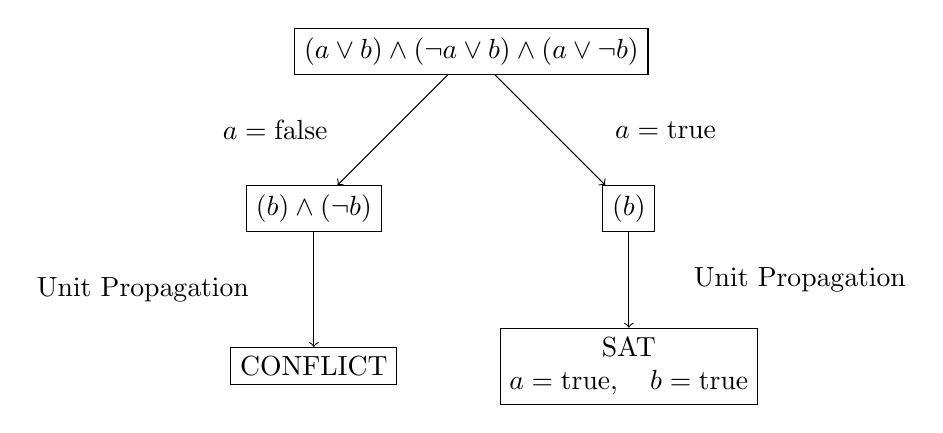
\begin{tikzpicture}
        \node[draw] (A) at (0,0)     {$(a \lor b) \land (\neg a \lor b) \land (a \lor \neg b)$};
        \node[draw] (B) at (-2,-2)   {$(b) \land (\neg b)$};
        \node[draw] (C) at (2,-2)    {$(b)$};
        \node[draw] (D) at (-2,-4) {CONFLICT};
        \node[draw, align=center] (E) at (2,-4)  {SAT \\ $a = \text{true},\quad b = \text{true}$};
        
        \draw[->]   (A) -- (B) node[midway, left=20pt] {$a = \text{false}$};
        \draw[->]   (A) -- (C) node[midway, right=20pt] {$a = \text{true}$};
        \draw[->]   (B) -- (D) node[midway, left=20pt] {Unit Propagation};
        \draw[->]   (C) -- (E) node[midway, right=20pt] {Unit Propagation};
    \end{tikzpicture}
    \caption{A run of DPLL on Equation \ref{eq:DP_example}}
    \label{fig:run_dpll}
\end{figure}

\subsection[CDCL]{Conflict Driven Clause Learning}
Recent competitive solvers are based on Conflict Driven Clause Learning (CDCL) \nomenclature[z-CDCL]{CDCL}{Conflict Driven CLause Learning}
\cite{SAT_Comp2017, sat2018descriptions}, such as Glucose.
CDCL builds on DPLL in a few ways, the key methods are as follows:

\begin{itemize}
    \item Derive new clauses when search yields a conflict \cite{marques1999grasp}.
    \item Use of efficient lazy data structures \cite{moskewicz2001chaff, ryan2004efficient}.
    \item Non-chronological backtracking \cite{marques1999grasp}.
    \item Restarting search \cite{gomes1998boosting, gomes2000heavy}
\end{itemize}

The structure of a CDCL solver without restarts can be seen in Algorithm \ref{alg:cdcl}.

\begin{algorithm}
\caption{Organisation of CDCL \cite{biere2009conflict, CDCL}}
\label{alg:cdcl}
\vspace{5pt}
\KwIn{CNF-SAT Formula $F$}
\KwOut{SAT or UNSAT}
\hrulefill\\

\nl $\alpha \gets \emptyset$ \\
\nl \If{unit\_propagation($F$, $\alpha$) == CONFLICT}
{
    \nl \Return{UNSAT} \\
}
\nl decision\_level $\gets 0$ \\
\nl \While{$\neg$ all\_variables\_assigned($F$, $\alpha$)}
{
    \nl $(x,v) \gets \text{pick\_branching\_variable}(F, \alpha)$ \\
    \nl decision\_level $\gets$ decision\_level $+ 1$ \\
    \nl $\alpha \gets \alpha \cup \{(x,v)\}$ \\
    \nl \If{unit\_propagation($F, \alpha$) == CONFLICT}
    {
        \nl $\beta \gets \text{conflict\_analysis}(F, \alpha)$ \\
        \nl \If{$\beta < 0$}
        {
            \nl \Return{UNSAT} \\
        }
        \nl \Else{
            \nl backtrack($F, \alpha, \beta$) \\
            \nl decision\_level $\gets \beta$ \\
        }
    }
}
\nl \Return{SAT}
\end{algorithm}

In Algorithm \ref{alg:cdcl} $\alpha$ refers to the set of assignments, where
each assignment is represented as a tuple $(x, v)$ where $x$ is a variable
and $v \in \{\text{false}, \text{true}\}$ is the value. The unit propagation
function call executes the one literal clause rule from Section \ref{sec:dpll}.
Pick branching variable chooses which variable to branch on and gives it a value.
Choice of heuristics for which variable to select is motivated mostly by which
features can be computed efficiently \cite{lewis2005speedup, moskewicz2001chaff}.

Backtrack takes in a parameter $\beta$, which indicates the decision level to
backtrack to. This means that search happens in a non-chronological fashion.
The level to backtrack to is decided by the conflict analysis function.
% This function looks at which clauses clauses the contradiction to occur
% and finds a clause implied by those clauses and adds it to the formula.
% The amount to backtrack by depends on what decision level the variables
% in the learned clause were assigned. One scheme involves always backtracking
% to the decision level of the most recently assigned variable \cite{biere2009conflict}.

\subsubsection{Conflict Analysis}
The most characteristic part of CDCL is the clause learning that results from the clause
analysis process. There are slight variants of this procedure, but we will cover the most
common variations popularised in GRASP \cite{marques1999grasp} and Chaff \cite{moskewicz2001chaff}.

For a particular partial assignment $\alpha$, we use decision level to mean the order that
a given variable was assigned by the \texttt{pick\_branching\_variable} routine. For
variables that were assigned via the \texttt{unit\_propagation} routine, they inherit the
highest decision level of the other variables in the clause. We consider a variable that
is assigned via \texttt{unit\_propagation} to be implied by the other variables in the unit clause.
Since \texttt{unit\_propagation} may lead to more clauses becoming unit, we can construct a directed
acyclic graph of implications. We call this graph the implication graph.

Consider the following boolean formula:
\begin{align}
    &(\neg x_1 \lor x_2 \lor x_4) \land (x_2 \lor \neg x_3 \lor \neg x_5) \land (\neg x_4 \lor x_5 \lor x_6) \nonumber \\
    \land &(\neg x_6 \lor x_7) \land (\neg x_3 \lor \neg x_6 \lor \neg x_8) \land (\neg x_7 \lor x_8) \label{eq:impl_ex}
\end{align}
For example, say that \texttt{pick\_branching\_variable} first assigns $x_1 = \text{true}$ at decision level 1, then
$x_3 = \text{true}$ at decision level 2 and then $x_2 = \text{false}$ at decision level 3. At this point, the first
two clauses in Equation \ref{eq:impl_ex} are unit clauses and applying \texttt{unit\_propagation} will lead to a conflict.
The resulting implication graph can be seen in Figure \ref{fig:implication_graph}. Each vertex represents an assignment
or a conflict and there is a directed edge from one vertex to another if that assignment implies the other via unit
propagation. For example, in Figure \ref{fig:implication_graph} there is an edge from $x_1 = \text{true}$ and $x_2 = \text{false}$
to $x_4 = \text{true}$ because the first two assignments make the clause $(\neg x_1 \lor x_2 \lor x_4)$ a unit clause which
implies $x_4 = \text{true}$. There are also edges from $x_7 = \text{true}$ and $x_8 = \text{false}$ to a conflict vertex since
these two assignments leave the clause $(\neg x_7 \lor x_8)$ unsatisfied. Each edge is labelled with the clause
that caused the implication.

\begin{figure}
    \centering
    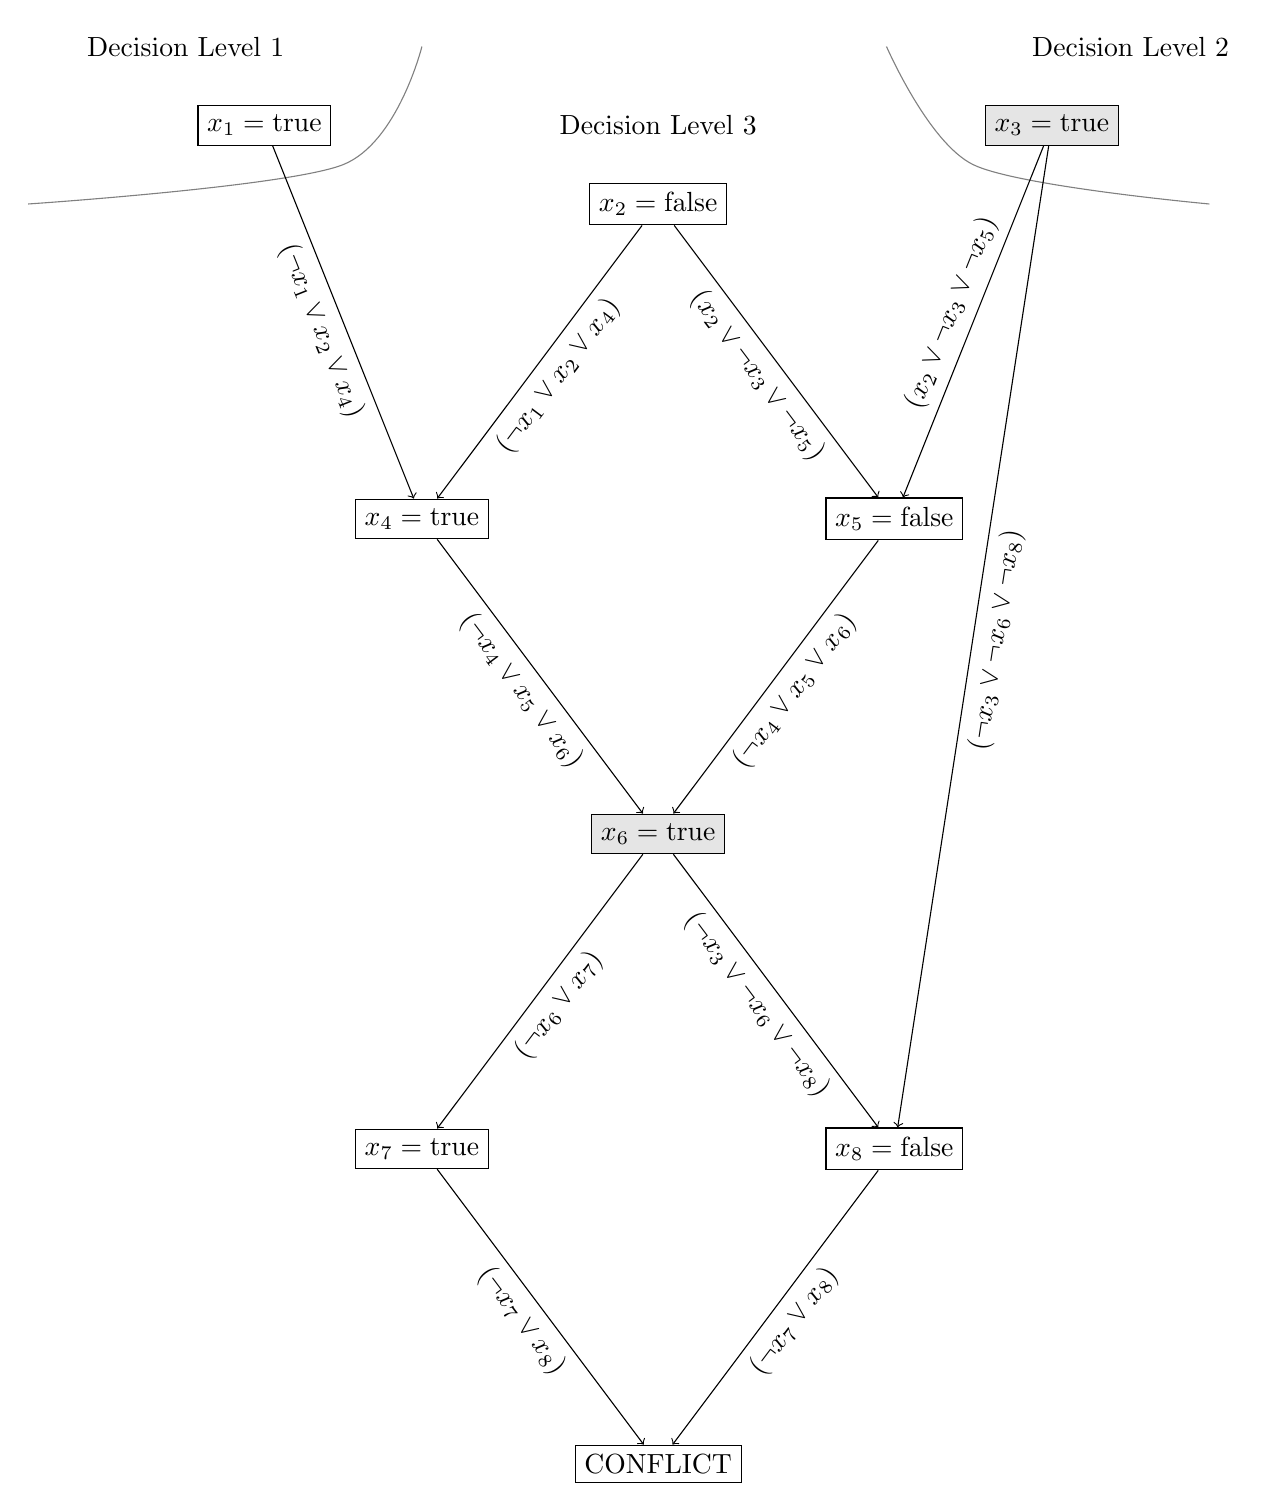
\begin{tikzpicture}
        \node[draw] (x1) at (-5, 1) {$x_1 = \text{true}$};
        \node[draw] (x2) at (0, 0) {$x_2 = \text{false}$};
        \node[draw, fill=black!10] (x3) at (5, 1) {$x_3 = \text{true}$};
        \node[draw] (x4) at (-3, -4) {$x_4 = \text{true}$};
        \node[draw] (x5) at (3, -4) {$x_5 = \text{false}$};
        \node[draw, fill=black!10] (x6) at (0, -8) {$x_6 = \text{true}$};
        \node[draw] (x7) at (-3, -12) {$x_7 = \text{true}$};
        \node[draw] (x8) at (3, -12) {$x_8 = \text{false}$};
        \node[draw] (k) at (0, -16) {CONFLICT};
        
        \draw[gray] plot [smooth] coordinates {(-8, 0) (-4, 0.5) (-3, 2)};
        \draw[gray] plot [smooth] coordinates {(7, 0) (4, 0.5) (2.9, 2)};
        \node[] (dl1) at (-6, 2) {Decision Level 1};
        \node[] (dl2) at (6, 2) {Decision Level 2};
        \node[] (dl3) at (0, 1) {Decision Level 3};
        
        \path[->] (x1) edge node[below, sloped] {$(\neg x_1 \lor x_2 \lor x_4)$} (x4);
        \path[->] (x2) edge node[below, sloped] {$(\neg x_1 \lor x_2 \lor x_4)$} (x4);
        \path[->] (x2) edge node[below, sloped] {$(x_2 \lor \neg x_3 \lor \neg x_5)$} (x5);
        \path[->] (x3) edge node[above, sloped] {$(x_2 \lor \neg x_3 \lor \neg x_5)$} (x5);
        \path[->] (x3) edge node[below, sloped] {$(\neg x_3 \lor \neg x_6 \lor \neg x_8)$} (x8);
        \path[->] (x4) edge node[below, sloped] {$(\neg x_4 \lor x_5 \lor x_6)$} (x6);
        \path[->] (x5) edge node[below, sloped] {$(\neg x_4 \lor x_5 \lor x_6)$} (x6);
        \path[->] (x6) edge node[below, sloped] {$(\neg x_6 \lor x_7)$} (x7);
        \path[->] (x6) edge node[below, sloped] {$(\neg x_3 \lor \neg x_6 \lor \neg x_8)$} (x8);
        \path[->] (x7) edge node[below, sloped] {$(\neg x_7 \lor x_8)$} (k);
        \path[->] (x8) edge node[below, sloped] {$(\neg x_7 \lor x_8)$} (k);
    \end{tikzpicture}
    \caption{Implication graph for Equation \ref{eq:impl_ex} for a partial assignment to $x_1, x_2, x_3$.
    First UIP is shaded grey}
    \label{fig:implication_graph}
\end{figure}

The \texttt{conflict\_analysis} routine will construct this implication graph and then apply
a number of resolution steps to obtain the learned clause. Define a resolution operator $\odot$ for
two clauses $C_1$ and $C_2$ with a unique variable $x_r$ such that $\neg x_r \in C_1$ and $x_r \in C_2$ or
vice versa, then $C_1 \odot C_2 = (C_1 \cup C_2) \setminus \{x_r, \neg x_r\}$ i.e. a clause containing
all literals in $C_1$ and $C_2$ excluding $x_r$ and $\neg x_r$. \texttt{conflict\_analysis} then begins by
taking the clause that caused the conflict (in this example $(\neg x_7 \lor x_8)$) and applying the resolution
operator with this clause and a clause that implied one of the literals in the first clause. In our example
the first resolution step could be either $(\neg x_7 \lor x_8) \odot (\neg x_6 \lor x_7) = (\neg x_6 \lor x_8)$ or 
$(\neg x_7 \lor x_8) \odot (\neg x_3 \lor \neg x_6 \neg x_8) = (\neg x_3 \lor \neg x_6 \lor \neg x_7)$.
A full set of resolution steps using the example from Equation \ref{eq:impl_ex} can be seen in Table \ref{tab:resolutions}.
Since $\forall C_1, C_2 \in F : C_1 \odot C_2 \approx C_1 \land C_2$ then $F \approx F \cup \{C_1 \odot C_2\}$. This means
that we can take any clause from Table \ref{tab:resolutions} and add it to Equation \ref{eq:impl_ex} without changing
its satisfiability.

\begin{table}[]
    \centering
    \begin{tabular}{l l}
    \toprule
        Step & Resolution \\
    \midrule
        1 & $(\neg x_7 \lor x_8) \odot (\neg x_6 \lor x_7) = (\neg x_6 \lor x_8)$ \\
        2 & $(\neg x_6 \lor x_8) \odot (\neg x_3 \lor \neg x_6 \lor \neg x_8) = (\neg x_3 \lor \neg x_6)$ \\
        3 & $(\neg x_3 \lor \neg x_6) \odot (\neg x_4 \lor x_5 \lor x_6) = (\neg x_3 \lor \neg x_4 \lor x_5)$ \\
        4 & $(\neg x_3 \lor \neg x_4 \lor x_5) \odot (x_2 \lor \neg x_3 \lor \neg x_5) = (x_2 \lor \neg x_3 \lor \neg x_4)$ \\
        5 & $(x_2 \lor \neg x_3 \lor \neg x_4) \odot (\neg x_1 \lor x_2 \lor x_4) = (\neg x_1 \lor x_2 \lor \neg x_3)$ \\
    \bottomrule
    \end{tabular}
    \caption{Resolution steps for Equation \ref{eq:impl_ex} with partial assignments to $x_1, x_2, x_3$}
    \label{tab:resolutions}
\end{table}

\nomenclature[z-UIP]{UIP}{Unit Implication Point}

There are different options for how many resolution steps to perform, however, a guiding principle is that the learned clause
should be as short as possible and should remain a unit clause after backtracking.
The most common approach is to stop at what is called the first Unit Implication Point (UIP) \cite{biere2009conflict}, which is the first point
at which there is only one literal in a learned clause that has the highest decision level. In Table \ref{tab:resolutions}
this occurs at step 2, since in the clause $(\neg x_3 \lor \neg x_6)$ only $x_6$ has decision level 3 while $x_3$
has decision level 2.
Note that if we look at the literals in a clause obtained by any number of resolution steps, the corresponding vertices
in the implication graph form a vertex separator, separating the side of the graph containing the conflict vertex
and the side containing the variables in the assignments made by \texttt{pick\_branching\_variable}. 
Therefore, we can interpret a UIP as a clause where the variable with the highest decision level
is a dominator for the variable most recently assigned by \texttt{pick\_branching\_variable}
with respect to the conflict vertex. This can be seen in Figure \ref{fig:implication_graph} as all paths from $x_2 = \text{false}$
to the conflict vertex must pass through $x_6 = \text{true}$.

The amount to backtrack by (given by $\beta$ in Algorithm \ref{alg:cdcl}) also varies from solver to solver
and most often depends on how inexpensive backtracking is given the datastructures used by the solver.
However, most modern solvers now use lazy datastructures which make it cheap to backtrack. For these
solvers a common approach is to backtrack until just before the learned clause no longer is a unit clause.
In the example given in Equation \ref{eq:impl_ex}, the learned clause was $(\neg x_3 \lor \neg x_6)$. As long
as $x_3$ remains assigned then the learned clause will be a unit clause, and $x_3$ was assigned at decision level 2,
so we can backtrack to decision level 2. In general we can backtrack to the second highest decision level in the
learned clause. This is the backtracking method used by Chaff \cite{moskewicz2001chaff}.
We can guarantee completeness because, since the learned clauses prevent the solver from exploring
the same assignment twice.

\subsubsection{Performance}

\begin{figure}
    \centering
    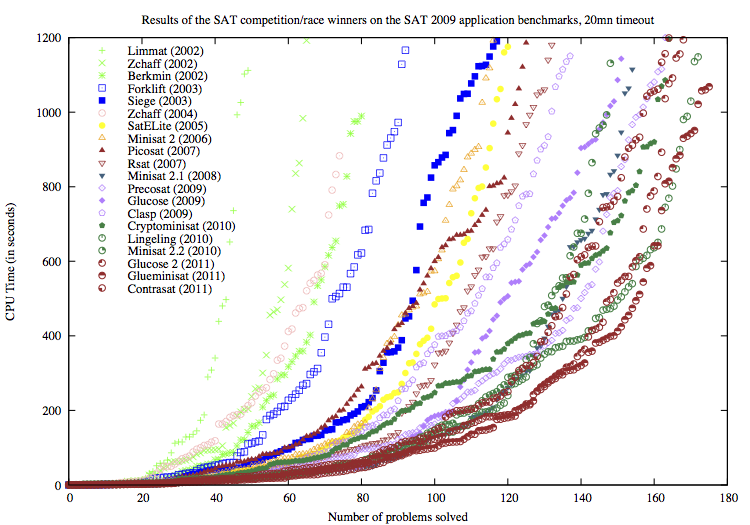
\includegraphics[scale=1]{sat_performance2012.png}
    \caption{Number of sat problems taken from the
    2009 SAT competition that were solved by various solvers
    with a 20 minute timeout \cite{sat2009theory}}
    \label{fig:sat_perf}
\end{figure}

In figure \ref{fig:sat_perf} we can see the number of solved instances of practical
sat benchmarks submitted to the 2009 SAT competition by various different solvers
\cite{sat2009theory}. Notably
more recent solvers, whilst still demonstrating exponential scaling behaviour are
able to solve significantly more problems than prior solvers.

For the 2018 SAT competition the benchmarks were taken from various different domains:
\cite{sat2018descriptions}

\begin{itemize}
    \item Proving the existence of a nonce for blockchain mining algorithms.
    \item Searching for a unit-distance graph with chromatic number 6 and k-colourability of graphs.
    \item Verifying simple floating-point programs.
    \item Cryptanalysis.
    \item Time-Slot allocation problems with optimal preference satisfaction
\end{itemize}

\subsection{Glucose}
Glucose is an efficient implementation of CDCL that has featured prominently
in many SAT competitions \cite{audemard2009glucose} building on top of MiniSAT \cite{een2003extensible}.
Glucose implements a few additional
features on top of CDCL, most prominently it implements new clause deletion policies
which help control the memory usage of the learned clauses generated by
the conflict analysis. These deletion policies expand on those used in the BerkMin solver \cite{goldberg2007berkmin},
going beyond analysing clauses just by size and how close they are to being a unit clause \cite{dechter1990enhancement, bayardo1997using}.

These policies were established in work by Audemard et al. where it is observed that
the decision level at which conflicts are encountered
tends to decrease as the solver progresses \cite{audemard2009predicting},
although this effect was only observed for ``industrial'' SAT instances.
This means that the solver is able to find conflicts faster over time, i.e.
it is assigning many variables via unit propagation. Additionally, this allows
for a crude estimate of when the solver will terminate.
Audemard et al. then devise a metric called the ``Literal
Block Distance'' (LBD) \nomenclature[z-LBD]{LBD}{Literal Block Distance}
which is the number of distinct decision levels in a clause
for a given assignment and show that when keeping only clauses with low LBD
the observation that decision levels decrease still holds. This suggests
that these clauses are the most important for allowing the solver to
spend significant time executing unit propagation.
Applying this deletion policy, around 93\% of learned clauses were deleted \cite{audemard2009glucose}.
However, since the learned clauses are needed for guaranteeing completeness, Glucose
is not complete.

Of practical note is that the Glucose solver is particularly
amenable to paralellisation and remains one of the most
competitive parallel solvers \cite{audemard2018glucose}.

\section{Stochastic Local Search Algorithms}
A different family of algorithms to backtracking algorithms is local search algorithms
which are based on the idea of randomly choosing an assignment and then making
small adjustments to assignment in order to try and find a satisfying assignment.
We will cover an important algorithm,
namely Sch\"oning's algorithm \cite{schoning1999probabilistic}, and then consider
WalkSat, a solver based on similar principles.

\subsection{Sch\"oning's Algorithm}

An interesting $k$-SAT algorithm that is able to beat the $\mathcal{O}^*(2^n)$
complexity for bounded $k$ is Sch\"oning's algorithm seen in Algorithm \ref{alg:schoning}.
Given that a satisfying assignment exists it will be found in expectation after
$(2 - \frac{2}{k})^n$ runs of Sch\"oning's algorithm \cite{schoning1999probabilistic}.
Hence the expected running time is $\mathcal{O}^*((2 - \frac{2}{k})^n)$.

\begin{algorithm}
\caption{Sch\"oning's Algorithm for $k$-SAT}\label{alg:schoning}
\vspace{5pt}
\KwIn{$k$-SAT instance, $F$}
\KwOut{Instance is satisfiable or not}
\hrulefill \\
\nl Guess initial assignment \\
\nl \For{$i \in \{1, \dots, 3n\}$}{
    \nl \If{$F$ is Satisfied}{
        \nl \Return{Accept} 
    }
    \nl \Else{
        \nl flip a random variable in an unsatisfied clause \\
    }
}
\end{algorithm}

\subsubsection{Analysis of Sch\"oning's Algorithm}
For the sake of brevity, we will only consider the case where $k=3$.
Since we require that there is at least one satisfying assignment let $\alpha^*$
be one such satisfying assignment. Let $\alpha$ be the assignment guessed in
the first line and let $d$ be the Hamming distance between $\alpha$ and $\alpha^*$,
i.e. $H(\alpha, \alpha^*) = d$ the number of variables in which they differ. The probability of guessing
an assignment $\alpha$ which differs by exactly $d$ variables from $\alpha^*$ is given by the following expression,
where $n$ is the number of variables.

\begin{equation}
    2^{-n}\binom{n}{d}
\end{equation}

If the algorithm flips a variable in which $\alpha$ and $\alpha^*$ differ, then
we call this a step towards the solution, i.e. $H(\alpha, \alpha^*)$ decreases by 1. Conversely, if they do not differ then
we call this a step away from the solution, i.e. $H(\alpha, \alpha^*)$ increases by 1.
%Let $T$ be the total number of steps,
%if a run of the algorithm where to find a satisfying assignment then we
%must have that the number of steps towards the solution must be
%$\frac{T + d}{2}$ and steps away must be $\frac{T - d}{2}$

Consider the probability of making $2d$ steps towards the solution
and $d$ steps away in the first $3d$ steps. It is clear that this will reach
$\alpha^*$ and since $d \leq n$, then the total number of steps 
will not be greater than $3n$. Since, in an unsatisfied clause,
at least one variable is different between $\alpha$ and $\alpha^*$, then when
the algorithm flips a random variable in that clause the probability of it
being one where the assignments are different is $\frac{1}{3}$. Hence,
the probability of making $2d$ toward the solution and $d$ steps away in the
first $3d$ steps is given by the following expression.

\begin{equation}
    \binom{3d}{d} \Big( \frac{1}{3} \Big)^{2d} \Big( \frac{2}{3} \Big)^d
\end{equation}

Hence to find the probability that the algorithm finds a satisfying solution
we simply have combine this with the probability of guessing a first assignment
that has Hamming distance of exactly $d$, and sum over all possible values of $d$.

\begin{equation} \label{eq:p_find_assignment}
    \mathrm{Pr}[\text{Find satisfying assignment}] = \sum_{d=0}^{n} 2^{-n}\binom{n}{d}\binom{3d}{d} \Big( \frac{1}{3} \Big)^{2d} \Big( \frac{2}{3} \Big)^d
\end{equation}

To simplify Equation \ref{eq:p_find_assignment} it will be helpful to consider
a lower bound of $\binom{3d}{d}$. To do this we will use Stirling's approximation
of the factorial:

\begin{equation} \label{eq:stirling_fac}
    n! \sim \sqrt{2\pi n} \Big( \frac{n}{e} \Big)^n
\end{equation}

Using Equation \ref{eq:stirling_fac} we can derive an approximation as follows.

\begin{align*}
    \binom{3d}{d} &= \frac{(3d)!}{(2d)! \cdot d!} \\[5pt]
    &\sim \frac{\sqrt{6 \pi d}\Big(\frac{3d}{e}\Big)^{3d}}{\sqrt{4\pi d} \Big( \frac{2d}{e} \Big)^{2d}\sqrt{2\pi d} \Big( \frac{d}{e} \Big)^d} \\[5pt]
    &\sim \frac{\sqrt{3}}{2\sqrt{\pi d}} \cdot \frac{3^{3d}}{2^{2d}}
\end{align*}

Since $n \geq d$ we replace $\sqrt{d}$ with $\sqrt{n}$ to simplify the analysis.
Then since the binomial coefficient is always strictly positive then what
remains is to choose a sufficiently large constant $\delta$
such that we have for $d \geq 0$:

\begin{equation} \label{eq:binom_bound}
    \binom{3d}{d} \geq \frac{1}{\delta \sqrt{n}} \cdot \frac{3^{3d}}{2^{2d}}
\end{equation}

Combining Equations \ref{eq:p_find_assignment} and \ref{eq:binom_bound} we get
a lower bound on the probability of finding a satisfying assignment.

\begin{align*}
    \mathrm{Pr}[\text{Find satisfying assignment}] &\geq \sum_{d=0}^{n} 2^{-n}\binom{n}{d} \frac{1}{\delta \sqrt{n}} \cdot \frac{3^{3d}}{2^{2d}} \Big( \frac{1}{3} \Big)^{2d} \Big( \frac{2}{3} \Big)^d \\[5pt]
    %&\geq \frac{2^{-n}}{\delta \sqrt{n}}\sum_{d=0}^{n} \binom{n}{d}\frac{3^{3d}}{2^{2d}} \frac{1}{3^{2d}} \frac{2^d}{3^d} \\[5pt]
    &\geq \frac{2^{-n}}{\delta \sqrt{n}}\sum_{d=0}^{n} \binom{n}{d}\frac{1}{2^{d}} \\[5pt]
    &\geq \frac{2^{-n}}{\delta \sqrt{n}}\Big( 1 + \frac{1}{2} \Big)^n \\[5pt]
    &\geq \frac{1}{\delta \sqrt{n}}\Big( \frac{3}{4} \Big)^n \\[5pt]
\end{align*}

Repeatedly running Algorithm \ref{alg:schoning} defines a geometric sequence.
Therefore, the expectation of the number of runs required to find the satisfying
assignment is given by

\begin{equation}
    \mathbb{E}[\text{\#runs}] = \frac{1}{\mathrm{Pr}[\text{Find satisfying assignment}]} \leq \delta\sqrt{n}\Big( \frac{4}{3} \Big)^n
\end{equation}

Hence the time complexity can be written as $\mathcal{O}^*(1.334^n)$.

\subsection{WalkSat}
WalkSat is an solver similar to Sch\"oning's algorithm that is inspired
by GSAT \cite{selman1992new, selman1994noise, selman1993local} and by ideas laid forth by Papadimitriou \cite{papadimitriou1991selecting}. The main difference between
WalkSat and Sch\"oning's algorithm is that it employs a semi-greedy
strategy when deciding which variable to flip in an unsatisfied clause.

With some probability $p$ WalkSat will flip a random variable, but
with probability $1 - p$ WalkSat will flip the variable that minimises
the number of clauses that become unsatisfied. The parameter $p$
is often called the noise parameter and optimal choice of $p$ depends
on the structure of the formula being tested. Therefore, modern improvements
have attempted to adapt $p$ automatically to each instance \cite{hoos2002adaptive}.

\begin{table}
    \centering
    \begin{tabular}{l l c c c}
    \toprule
        \multicolumn{2}{l}{Formula} & DP Time & GSAT Time & WalkSat Time \\
        \#Vars & \#Clauses & & & \\
        \midrule
        708 & 1702 & * & 0.081 & 0.013 \\
        649 & 1562 & * & 0.058 & 0.014 \\
        8704 & 32316 & * & 94.1 & 1.0 \\
        8432 & 31310 & * & 456.6 & 0.7 \\
        300 & 730 & 23096 & 0.009 & 0.002 \\
        125 & 310 & 1.4 & 0.009 & 0.001 \\
        \bottomrule
    \end{tabular}
    \caption[Comparing DP, GSAT and WalkSat]
    {Comparing solution times of an implementation of
    the Davis Putnam procedure (DP) with GSAT and WalkSat 
    (time in seconds) \cite{selman1993local}}
    \label{tab:walksat_times}
\end{table}

WalkSat is an efficient solver that is able to tackle SAT instances with a large
number of variables and clauses, and is able to find solutions to instances
where an efficient implementation of the Davis Putnam procedure was unable
to a find a solution. An overview of solution times for a few SAT benchmark
problems from 1993 is seen in Table \ref{tab:walksat_times}.
%!TEX root = ../thesis.tex
%*******************************************************************************
%****************************** Third Chapter **********************************
%*******************************************************************************
\chapter{Complexity Conjectures} \label{chap:complexity}

% **************************** Define Graphics Path **************************
\ifpdf
    \graphicspath{{Chapter3/Figs/Raster/}{Chapter3/Figs/PDF/}{Chapter3/Figs/}}
\else
    \graphicspath{{Chapter3/Figs/Vector/}{Chapter3/Figs/}}
\fi

\section{Exponential Time Hypothesis}
Of all the algorithms covered in the previous chapter, they all had exponential computational
time complexity, with all of the backtracking based algorithms requiring $\mathcal{O}^*(2^n)$ in the worst case. Slightly better was
Sch\"oning's Algorithm \ref{alg:schoning}, which had a complexity of
$\mathcal{O}^*((2 - \frac{2}{k})^n)$. However, for a general formula in CNF
$k$ could be arbitrarily large and as $k \to \infty$ then we recover the same
complexity as the other algorithms. So even when considering the case where we
have a 3SAT instance, we are unable to improve over the
exponential complexity.

\nomenclature[x-Ostar]{$\mathcal{O}^{\ast}(\cdot)$}{Big-O ignoring polynomial factors}

We know that $k$-SAT is NP-COMPLETE for $k \geq 3$\cite{schaefer1978complexity},
so unless $P = NP$ we should not expect to find a polynomial time algorithm.
However, it is still theoretically possible, under the assumption that $P \neq NP$, for there to exist an algorithm which is superpolynomial but subexponential.
Here we say that $f(x)$ is subexponential if it is $\mathcal{O}^{\ast}(2^{\epsilon n})$ for all
$\epsilon > 0, \quad \epsilon \in \mathbb{R}$ with $\mathcal{O}^{\ast}(g(x))$ meaning $\mathcal{O}(poly(n) \cdot g(x))$,
i.e. ignoring polynomial factors. Such an algorithm
could have running time $T(n) = \mathcal{O}^{\ast}(2^{\frac{n}{\log n}})$ which is 
$\mathcal{O}^{\ast}(2^{\epsilon n}),\quad \epsilon > 0$.
However, no such algorithm for SAT has been found.

Due to the seeming difficulty of finding significantly faster $k$-SAT algorithms
there have been two conjectures
put forward by Impagliazzo and Paturi, which
relate to the complexity of $k$-SAT. These are the ``Exponential Time Hypothesis'' and the ``Strong
Exponential Time Hypothesis'', abbreviated to ETH and SETH respectively \cite{impagliazzo2001complexity}.

\nomenclature[z-ETH]{ETH}{Exponential Time Hypothesis}
\nomenclature[z-SETH]{SETH}{Strong Exponential Time Hypothesis}

Informally ETH hypothesises that there does not exist a subexponential time algorithm solving SAT.
More formally, consider the set of all $k$-SAT algorithms and
express their time complexities in the form $\mathcal{O}^{\ast}(2^{\delta n})$
for some constant $\delta \in \mathbb{R}^{+} \cup \{0\}$.
Then for $k \in \mathbb{N}, \quad k \geq 3$ let $s_k$ be the infimum
of $\delta$s taken from this set
\begin{equation} \label{eq:ETH}
    s_k = \inf \{\delta: \text{$k$-SAT is solvable in time } \mathcal{O}^{\ast}(2^{\delta n})\}
\end{equation}
The ETH then states that $s_{3} > 0$ \cite{impagliazzo2001complexity}.
Intuitively this means that there must exist some non-zero constant $s_{3}$ such
that solving 3-SAT takes time $\Omega^{\ast}(2^{s_{3} n})$ which rules out
a subexponential time algorithm for 3-SAT.
The statement that $s_3 > 0$ is equivalent to the statement that
for all $k \in \mathbb{N}$ if $k \geq 3$ then $s_k > 0$,
i.e. there then cannot exist a subexponential time
algorithm for $k$-SAT with $k \geq 3$. This is because a 3-CNF can be easily
reduced to a $k$-CNF for all $k \geq 3$.

If we, instead of considering all $k$-SAT algorithms, consider just Sch\"oning's
algorithm, then we get a new sequence of $s'_k$ where 
$\forall k \in \mathbb{N}: s'_k \geq s_k$. Rearranging the complexity
of Sch\"oning's algorithm we get that

\begin{equation} \label{eq:sk_schoing}
    s'_k = \log_2(2 - \frac{2}{k}), \quad k \geq 3
\end{equation}

which yields the sequence $\sim 0.415, \sim 0.585, \sim 0.678, \dots$ for
$k= 3,4,5, \dots$. It is clear from Equation \ref{eq:sk_schoing} that
as $k \to \infty$ then $s'_k \to 1$.
There are known algorithms that produce smaller constants \cite{hofmeister2002probabilistic},
however these algorithms still generate a sequence that tends to 1 as
$k \to \infty$.

The ``Strong Exponential Time Hypothesis'' (SETH) considers this limit
as $k$ tends to infinity. SETH states that
\begin{equation} \label{eq:SETH}
    \lim_{k \to \infty} s_{k} = 1
\end{equation}
Intuitively, if SETH were proven true,
this would mean that for general SAT there is no algorithm that is
asymptotically faster than brute force search and algorithms
such as DP, DPLL and CDCL would be optimal up to subexponential factors.
% highlight any differences between the formalism and the intuition

\subsection{Conditional Lower Bounds}
The ETH and SETH both imply that $P \neq NP$, so we should not hope to
prove either conjecture just yet. However, we can consider the implications
that these conjectures would have on other problems if they were proven true.
This allows for us to show that many problems have conditional lower bounds
on their complexity and for many problems that current algorithms
are optimal assuming one of these conjectures.

If we consider attempting to show lower bounds from an assumption of the ETH,
then since the ETH deals with the non-existence of subexponential time algorithms
for $k$-SAT, we could hope to reduce $k$-SAT to a number of different problems in
such a way that preserves subexponential time.

Since we are dealing with parameterized complexities for $k$-SAT with parameters
$n$ and $m$, when considering general problems we will use the mapping
$\kappa: \Sigma^* \mapsto \mathbb{N}$ to denote the parameter an instance
of the problem $x \in \Sigma^*$. Where $\Sigma^*$ is the set of problem instances.

\begin{definition}
    A Turing reduction from a problem $(A_1, \kappa_1)$ to a problem
    $(A_2, \kappa_2)$ is considered a SERF-T reduction if
    \begin{enumerate}
        \item The reduction on an instance $x$ of $A_1$
        runs in time $\mathcal{O}(2^{\epsilon \kappa_1(x)}|x|^{\mathcal{O}(1)})$
        for a choice of $\epsilon > 0$.
        \item For a query to $A_2$ with input $x'$:
        \begin{enumerate}
            \item $|x'| \leq |x|^{\mathcal{O}(1)}$
            \item $\kappa_2(x') \leq \alpha \kappa_1(x)$
        \end{enumerate}
        Where the constants hidden in the $\mathcal{O}(\cdot)$ do not
        depend on the choice of $\epsilon$.
        The constant $\alpha$ may depend on $\epsilon$
    \end{enumerate}
\end{definition}

To see how this works, consider two parameterized problems $(A_1, \kappa_1)$
and $(A_2, \kappa_2)$, where the second problem has a parameterized
subexponential time algorithm. We wish to show that if $(A_1, \kappa_1)$ is
SERF-T reducible to $(A_2, \kappa_2)$ then there also exists a parameterized
subexponential time algorithm for $(A_1, \kappa_1)$, i.e. for a choice of
$\epsilon > 0$ we need to show that $(A_1, \kappa_1)$ runs in time
$\mathcal{O}(2^{\epsilon \kappa_1(x)}|x|^{\mathcal{O}(1)})$.

Do show this, choose an $\epsilon > 0$.
Let $\epsilon' = \frac{\epsilon}{2}$ and run the SERF-T reduction
with parameter $\epsilon'$. Since this reduction runs in time
$\mathcal{O}(2^{\epsilon' \kappa_1(x)}|x|^{\mathcal{O}(1)})$ then this bounds
the number of calls to $(A_2, \kappa_2)$ by the same amount.
Each call to $(A_2, \kappa_2)$ has an instance $|x'| \leq |x|^{\mathcal{O}(1)}$
and $\kappa_2(x') \leq \alpha \kappa_1(x)$.
Since, from our assumption that $(A_2, \kappa_2)$ runs in parameterized subexponential
time we can choose $\epsilon'' = \frac{\epsilon'}{\alpha}$ and then each call to $(A_2, \kappa_2)$ can be made to run in time 
\begin{equation}
    \mathcal{O}(2^{\epsilon' \kappa_1(x)}|x|^{\mathcal{O}(1)})
\end{equation}
Therefore, the total time for solving $(A_1, \kappa_1)$ is given by
\begin{equation}
    \mathcal{O}(2^{\epsilon' \kappa_1(x)}|x|^{\mathcal{O}(1)}) \cdot
    \mathcal{O}(2^{\epsilon' \kappa_1(x)}|x|^{\mathcal{O}(1)}) =
    \mathcal{O}(2^{\epsilon \kappa_1(x)}|x|^{\mathcal{O}(1)})
\end{equation}
which is what we wanted to show. \cite{lokshtanov2013lower}

\subsubsection{Lower Bounds for 3-colouring}

To show that ETH implies that there is no subexponential time algorithm for 3-colourability
we must show that the standard reduction from 3-SAT to 3-colourability is also
a SERF-T reduction. The first requirement that the reduction runs in time 
$\mathcal{O}(2^{\epsilon \kappa_1(x)}|x|^{\mathcal{O}(1)})$ for all $\epsilon > 0$ is trivially
satisfied since the reduction runs in polynomial time.
Hence it also follows that the reduced instance $|x'| \leq |x|^{\mathcal{O}(1)}$.

Thus, the only thing left to show is that $\kappa_2(x') \leq \alpha \kappa_1(x)$ for
some constant $\alpha$. In this case $\kappa_2(x')$ would be the number of vertices
in the reduced instance and $\kappa_1(x) = n$.

To do this, recall the the standard reduction reduction from 3-SAT to 3-colourability
(see Figure \ref{fig:reduce_3col}).
We have a triangle and label the vertices as True, False and Base.
For each variable $x_i$ we create vertices labelled $x_i$ and $\neg x_i$ and
edges $(x_i, \neg x_i), (x_i, \text{Base}), (\neg x_i, \text{Base})$. Then
for each clause we have two ``or'' gadgets that consist of 3 vertices.
Thus, the total number of vertices in the instance $x'$ is given by
\begin{equation}
    \kappa_2(x') = 2n + 3m + 3
\end{equation}
This appears to be an issue, since we are unable to make $\kappa_2(x')$ linear in $n$
since $m$ could be a superlinear function of $n$ for an arbitrary instance of 3-SAT $x$.
However, we can make use of the sparsification lemma \cite{impagliazzo2001problems} to
reduce any $k$-SAT instance into a subexponential number of $k$-SAT instances where
$m$ is linear in $n$ and this takes subexponential time. We will detail the
sparsification lemma in Chapter \ref{chap:sparsication}.

Hence, to get our SERF-T reduction we first apply the sparsification lemma to
reduce our original instance $x$ into subexponentially many new $k$-SAT instances
and apply our standard 3-SAT to 3-colourability reduction to each new instance.
Since we can now guarantee that $m$ is $\mathcal{O}(n)$ then $2n + 3m + 3$ is also
$\mathcal{O}(n)$. We let $\alpha$ be the constant hidden in the $\mathcal{O}(\cdot)$.
Since the sparsification lemma produces a subexponential number of instances that
are no longer than the original instance and since it runs in subexponential time, then
we do not violate the time constraints of the SERF-T reduction.

Hence we have shown that this reduction satisfies all the requirements of a SERF-T
requirement. We can therefore say that if 3-colourability on $|V|$ vertices can
be solved in time $\mathcal{O}^{\ast}(2^{\epsilon \cdot |V|})$ for all $\epsilon > 0$
then 3-SAT could be solved in time $\mathcal{O}^{\ast}(2^{\epsilon \cdot n})$ 
for all $\epsilon > 0$, which would violate the ETH.

\begin{figure}
    \centering
    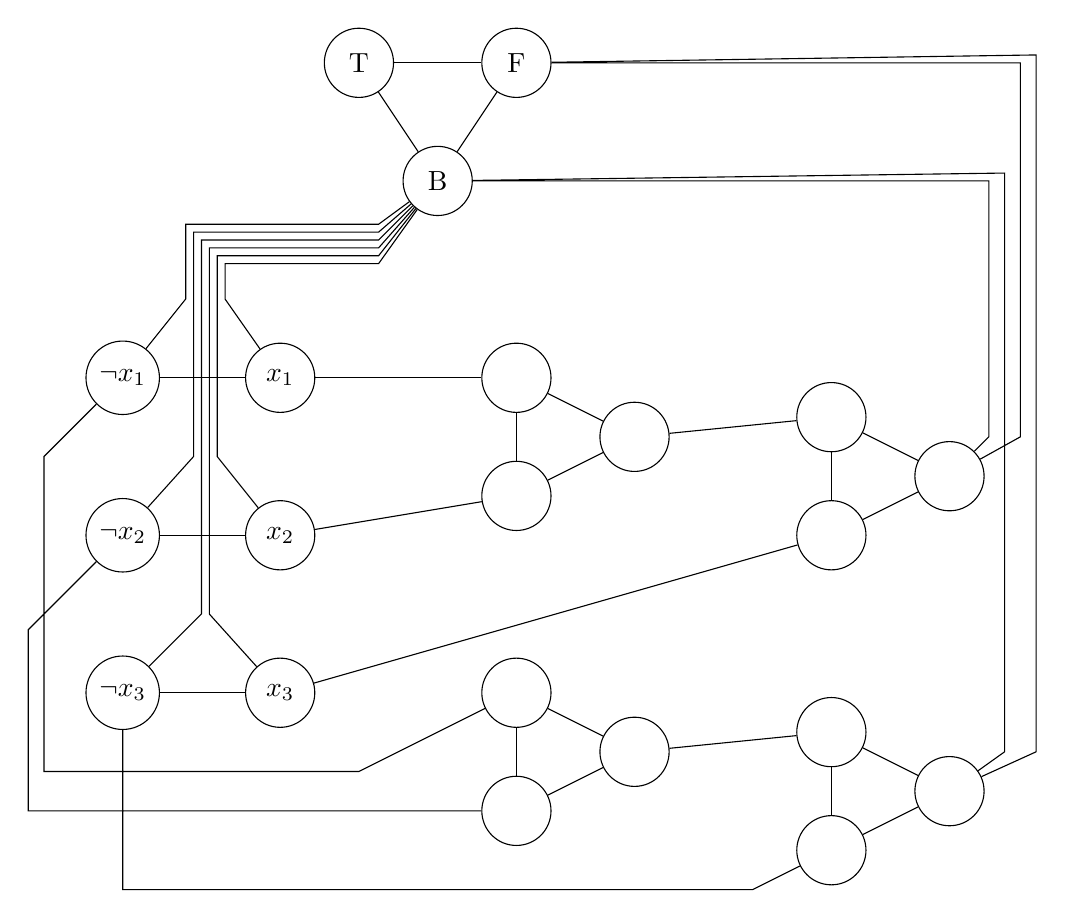
\begin{tikzpicture}
        \begin{scope}[auto,every node/.style={draw,circle,minimum size=2.5em}]
        % Pallet
        \node (T) at (-1,0) {T};
        \node (F) at (1,0) {F};
        \node (B) at (0,-1.5) {B};
        
        % Variables
        \node (x1) at (-2, -4) {$x_1$};
        \node (!x1) at (-4, -4) {$\neg x_1$};
        \node (x2) at (-2, -6) {$x_2$};
        \node (!x2) at (-4, -6) {$\neg x_2$};
        \node (x3) at (-2, -8) {$x_3$};
        \node (!x3) at (-4, -8) {$\neg x_3$};
        
        % Or gadets
        \node (or1a) at (1, -4) {};
        \node (or1b) at (2.5, -4.75) {};
        \node (or1c) at (1, -5.5) {};
        
        \node (or2a) at (5, -4.5) {};
        \node (or2b) at (6.5, -5.25) {};
        \node (or2c) at (5, -6) {};
        
        \node (or3a) at (1, -8) {};
        \node (or3b) at (2.5, -8.75) {};
        \node (or3c) at (1, -9.5) {};
        
        \node (or4a) at (5, -8.5) {};
        \node (or4b) at (6.5, -9.25) {};
        \node (or4c) at (5, -10) {};
        \end{scope}
        
        \path (T) edge (F) edge (B)
              (B) edge (F)
              (!x1) edge (x1)
              (!x2) edge (x2)
              (!x3) edge (x3)
              (or1a) edge (or1b)
              (or1b) edge (or1c)
              (or1c) edge (or1a)
              (or2a) edge (or2b)
              (or2b) edge (or2c)
              (or2c) edge (or2a)
              (or3a) edge (or3b)
              (or3b) edge (or3c)
              (or3c) edge (or3a)
              (or4a) edge (or4b)
              (or4b) edge (or4c)
              (or4c) edge (or4a)
              (x1) edge (or1a)
              (x2) edge (or1c)
              (or1b) edge (or2a)
              (x3) edge (or2c);
              
        \draw (!x1) -- (-5, -5) -- (-5 , -9) -- (-1, -9) -- (or3a)
              (!x2) -- (-5.2, -7.2) -- (-5.2, -9.5) -- (or3c)
              (or3b) -- (or4a)
              (!x3) -- (-4, -10.5) -- (4, -10.5) -- (or4c)
              (or2b) -- (7, -4.75) -- (7, -1.5) -- (B)
              (or2b) -- (7.4, -4.75) -- (7.4, 0) -- (F)
              (or4b) -- (7.2, -8.75) -- (7.2, -1.4) -- (B)
              (or4b) -- (7.6, -8.75) -- (7.6, 0.1) -- (F)
              (B) -- (-0.75, -2.25) -- (-3, -2.25) -- (-3, -7) -- (!x3)
              (B) -- (-0.75, -2.35) -- (-2.9, -2.35) -- (-2.9, -7) -- (x3)
              (B) -- (-0.75, -2.15) -- (-3.1, -2.15) -- (-3.1, -5) -- (!x2)
              (B) -- (-0.75, -2.45) -- (-2.8, -2.45) -- (-2.8, -5) -- (x2)
              (B) -- (-0.75, -2.05) -- (-3.2, -2.05) -- (-3.2, -3) -- (!x1)
              (B) -- (-0.75, -2.55) -- (-2.7, -2.55) -- (-2.7, -3) -- (x1);
        
    \end{tikzpicture}
    \caption[Reduction to 3-colourability]{Standard reduction of 
    $(x_1 \lor x_2 \lor x_3) \land (\neg x_1 \lor \neg x_2 \lor \neg x_3)$ to 3-colourability}
    \label{fig:reduce_3col}
\end{figure}

Using similar techniques we can also establish that the ETH implies that
there are no subexponential time algorithms for the following \cite{lokshtanov2013lower}.
\begin{itemize}
    \item Independent Set
    \item Dominating Set
    \item Vertex Cover
    \item Hamiltonian Path
\end{itemize}

\subsubsection{Lower Bounds for Planar Graph Problems}
Note that the SERF-T reduction from 3-SAT to 3-colourability depended on the
fact that the number of vertices in the
3-colourability instance was linear in the in the number of variables
in the 3-SAT instance. Typically for planar graph problems, this
property cannot be obtained.

For instance the reduction from 3-SAT to planar hamiltonian cycle 
creates a graph $G$ where the number of vertices is $\mathcal{O}(m^2)$ \cite{garey1976planar}.
As such we cannot establish a SERF-T reduction from 3-SAT to planar hamiltonian cycle 
parameterized by the number of vertices.
However, if we let the parameter be $\kappa_2(x') = \sqrt{|V|}$, then it is obvious that
this parameter is $\mathcal{O}(m)$. Then we can use the same techniques as before to
establish that the ETH implies that there is no $2^{o(\sqrt{|V|})}$ algorithm for planar
hamiltonian cycle.

The same argument can be made for many planar graph problems. Taken in conjunction
with algorithms using the planar separator theorem \cite{lipton1979separator} this
then means that many planar graph algorithms are optimal \cite{lipton1977applications}.

\subsection{Further Conditional Lower Bounds for Algorithms in P}
Proofs of conditional lower bounds are not limited to problems that
have superpolynomial complexities. Here we will give an example
of a lower bound for the orthogonal vectors problem based on the assumption
of the SETH \cite{williams2004new}.

\begin{definition}
    The orthogonal vectors problem is, given two sets $U$ and $V$ of bit vectors of length
    $d$ where $|U| = |V| = n$ and $d$ is $\omega(\log n)$, does there exist $u \in U$ and
    $v \in V$ such that $\sum_{i = 1}^{d} u_i \cdot v_i = 0$
\end{definition}

Best known algorithms for orthogonal vectors take time $\mathcal{O}(n^{2 - o(1)})$ and
it is unknown whether there is any ``strongly subquadratic'' algorithm, i.e. an
algorithm taking time $\mathcal{O}(n^{2 - \epsilon})$ for some $\epsilon > 0$. However,
Williams et al. show that SETH implies that no such algorithm exists \cite{williams2004new}.

To show this we will need the concept a fine grained reduction. Such a reduction
has the property that for two problems $A$ and $B$ with best known running times
$a(n)$ and $b(n)$ respectively, an improvement on $B$ to $\mathcal{O}(b(n)^{1 - \epsilon})$
leads to an improvement on $A$ to $\mathcal{O}(a(n)^{1 - \delta})$ for all $\epsilon > 0$
and some $\delta > 0$. Such a reduction is often denoted as a $(a(n), b(n))$-reduction \cite{vassilevska2015hardness}

\begin{definition}
    A fine grained reduction $M$ from problem $A$ to problem $B$ with running times
    $a(n)$ and $b(n)$ respectively obeys the following:
    For all $\epsilon > 0$, there is some $\delta > 0$ and some constant $d$
    such that for all $n \geq 1$ there is some constant $k_n$ and
    \begin{itemize}
        \item $M$ runs in time $d \cdot (a(n))^{1 - \delta}$,
        \item $M$ produces at most $k_n$ instances of $B$ adaptively,
        \item $\sum_{i = 1}^{k_n}(b(n'_i)^{1 - \epsilon}) \leq d \cdot (a(n))^{1 - \delta}$, where $n'_i$ is the
        $i_{\text{th}}$ instance of $B$. 
    \end{itemize}
    Instance sizes $n'_i$ may depend on $n$ and $\epsilon$, but $d$ can depend only on $\epsilon$ and not on $n$.
\end{definition}

The $(2^n, n^2)$-reduction from $k$-SAT to orthogonal vectors is then as follows. Apply the sparsification lemma
to the $k$-SAT instance, then partition the variables arbitrarily into two sets $D_1, D_2$ such
that each set contains $\frac{n}{2}$ variables. Construct two sets of vectors $U_1, U_2$ as follows:
For all $i \in \{1,2\}$ and for all assignments $\alpha$ to the variables in $D_i$, $v_{i, \alpha} \in U_i$
where for all clauses $C$, $v_{i, \alpha}[C] = 0$ if and only if the clause $C$ is satisfied by the
assignment $\alpha$ to the variables in $D_i$, $1$ otherwise. Therefore, if two vectors are orthogonal then
there exists an assignment to the variables in $D_1$ and $D_2$ such that for every clause it
is either satisfied by the assignment to $D_1$ or the assignment to $D_2$ \cite{williams2004new}.

Hence, any $\mathcal{O}(n^{2 - \epsilon})$ time algorithm for orthogonal vectors implies that there
is a $\mathcal{O}(2^{(1 - \delta)n})$ algorithm for $k$-SAT for all $k$. Therefore, the SETH
implies that there cannot be such an algorithm for orthogonal vectors.

Applying similar techniques, SETH implies
\begin{itemize}
    \item Fr\'echet distance cannot be computed in $\mathcal{O}(n^{2 - \epsilon})$ \cite{bringmann2014walking}
    \item Edit distance cannot be computed in $\mathcal{O}(n^{2 - \epsilon})$ \cite{backurs2015edit}
    \item Dynamic Time Warping distance cannot be computed in $\mathcal{O}(n^{2 - \epsilon})$ \cite{bringmann2015quadratic}
    \item Longest Common Subsequence cannot be computed in $\mathcal{O}(n^{2 - \epsilon})$ \cite{bringmann2018multivariate, polak2018hard}
\end{itemize}
%!TEX root = ../thesis.tex
%*******************************************************************************
%****************************** Third Chapter **********************************
%*******************************************************************************
\chapter{Sparsification Lemma} \label{chap:sparsication}

% **************************** Define Graphics Path **************************
\ifpdf
    \graphicspath{{Chapter4/Figs/Raster/}{Chapter4/Figs/PDF/}{Chapter4/Figs/}}
\else
    \graphicspath{{Chapter4/Figs/Vector/}{Chapte4/Figs/}}
\fi



\section*{Introduction}
% State how it would be used
In this chapter we will explain the sparsification lemma that allowed
us to show lower bounds on problems in $P$ conditioned on the SETH in Chapter \ref{chap:complexity}.
To do this we will first consider an example problem which again motivates the need
for the sparsification lemma. The example is the following.
Recall the definition of $s_k$ from Equation \ref{eq:ETH}.
\begin{theorem}
    If there exists a $k \geq 3$ such that $s_k > 0$, then $s_3 > 0$ \cite{impagliazzo2001complexity}.
\end{theorem}
To show this, we would have to prove that if there are no subexponential
time algorithms for $k$-SAT for some $k > 3$ then there is no subexponential algorithm for 3-SAT.
To make things simpler, we will show the contrapositive, that if there is a subexponential time algorithm
for 3-SAT then there is a subexponential time algorithm for $k$-SAT for all $k \geq 3$.

Assume then that we have an algorithm $A$ that solves 3-SAT in subexponential time
i.e. it takes $\mathcal{O}^{\ast}(2^{\epsilon n})$ time and we want to solve an
instance of $k$-SAT where $k > 3$. We can attempt to solve this
instance via a reduction to 3-SAT.
To reduce k-SAT to 3-SAT consider a k-CNF formula $F_{k}$ and consider a specific clause
$C = (x_{1} \lor x_{2} \lor \ldots \lor x_{k})$ from $F_k$. We will then introduce new variables
$y_{1}, y_{2}, \ldots, y_{k-3}$ and define $k-2$ new clauses as follows:

\begin{align*}
C'_{1} &= (x_{1} \lor x_{2} \lor y_{1}) \\
C'_{2} &= (\overline{y_{1}} \lor x_{3} \lor y_{2}) \\
C'_{3} &= (\overline{y_{2}} \lor x_{4} \lor y_{3}) \\
&\hspace{30pt}\vdots \\
C'_{k-2} &= (\overline{y_{k-3}} \lor x_{k-1} \lor x_{k})
\end{align*}

Observe that the conjunction of the clauses $C'_{1}, C'_{2}, \dots, C'_{k-2}$
is satisfiable if and only if the original clause $C$ is satisfiable.
This procedure can then be repeated for all clauses in $F_{k}$ to convert
the $k$-SAT formula with $n$ variables and $m$ clauses to a 3-SAT formula with $n + (k-3)m$ variables
and $(k-2)m$ clauses.
If we now use algorithm $A$, then we solve the instance in time $\mathcal{O}^{\ast}(2^{\epsilon \cdot (n + (k - 3)m)})$.
This is an issue, if we consider the fact that for an arbitrary $k$-SAT formula the number of
clauses could be significantly larger than the number of variables. Consider the case where $m = n^2$.
This then means that $A$ would run in time $2^{\mathcal{O}(n^2)}$ which is certainly not subexponential.

Fundamentally, the issue is that the reduction introduced too many new variables and these new variables
came from the number of clauses in the original formula. If we could guarantee that the number of
clauses in original formula was linear in the number of variables, i.e. $m = \mathcal{O}(n)$,
then the reduction would work.

\section{Statement of the lemma}
% State the lemma
The sparsification lemma as stated by Impagliazzo, Paturi and Zane originally relates to
$k$-Set Cover, from which they derive the k-SAT version as a corollary \cite{impagliazzo2001problems}.
The original formulation is stated here for completeness. Note that although this problem is called
$k$-Set Cover by Impagliazzo et al. \cite{impagliazzo2001problems}, it is typically refered to as $k$-Hitting Set.

An instance of $k$-Set Cover has a universe of $n$ elements $x_1, x_2, \dots, x_n$ and a collection $\mathcal{S}$
of subsets $S \subseteq \{x_1, x_2, \dots, x_n\}$. However, $\forall S \in \mathcal{S} : |S| \leq k$.
A $k$-set cover is a set $C \subseteq \{x_1, x_2, \dots, x_n\}$ such that $\forall S \in \mathcal{S} : S \cap C \neq \emptyset$.
Let $\sigma(\mathcal{S})$ be the collection of all such sets that cover $\mathcal{S}$. The goal is to find a minimal size $k$-set cover.
Let $\mathcal{T}$ be a restriction on $\mathcal{S}$ if for each $S \in \mathcal{S}$ there is a $T \in \mathcal{T}$ such that $T \subseteq S$.

\begin{theorem} \label{thm:kset_sparse}
    (Sparsification Lemma for $k$-Set Cover)
    For all $\epsilon > 0$ and $k \in \mathbb{N}^{+}$ there is a constant $C$ and an algorithm that given an instance $\mathcal{S}$
    of $k$-Set Cover on a universe of size n, produced a list of $t \leq 2^{\epsilon n}$ restrictions $\mathcal{T}_1, \mathcal{T}_2, \dots, \mathcal{T}_t$
    of $\mathcal{S}$ so that $\sigma(\mathcal{S}) = \bigcup_{i = 1}^{t} \sigma(\mathcal{T}_i)$ and so that $\forall i: |\mathcal{T}_i| \leq Cn$.
    Additionally the algorithm runs in time $\mathcal{O}^{\ast}(2^{\epsilon n})$ \cite{impagliazzo2001problems}.
\end{theorem}

This essentially states that for each $k$ and $\epsilon$ there exists an algorithm that can compute a subexponential number
of new collections such that each new collection contains a number of subsets linear in $n$.
The corollary for k-SAT can be obtained by considering the universe of elements in $k$-Set Cover to be
the $2n$ literals in the formula. $\mathcal{S}$ is then the formula with each $S \in \mathcal{S}$ being a clause.
We also require an additional set for each variable, $\{x_i, \overline{x_i}\}$, thus every cover of size exactly $n$
covers exactly one literal for each variable. Each restriction $\mathcal{T}_i$ can be thought of as a subformula of $\mathcal{S}$.

\begin{corollary} \label{cor:ksat_sparse}
    (Sparsification Lemma for $k$-SAT)
    For all $k \in \mathbb{N}^{+}$ and $\epsilon > 0$ there exists an algorithm that takes in a $k$-CNF formula $F$
    with $n$ variables and $m$ clauses and returns a collection of $k$-CNF formulas 
    $F'_1, F'_2, \dots, F'_t$, with the following properties.
    \begin{enumerate}
        \item $F$ is satisfiable if and only if $\bigvee_{i=1}^{t} F'_i$ is satisfiable.
        \item $F'_i$ has no more variables than $F$
        \item Number of clauses in $F'_i$ is less than $c(k, \epsilon)n$, where $c(k, \epsilon)$
        is a constant that does not depend on $n$.
        \item The algorithm takes time $\mathcal{O}^{\ast}(2^{\epsilon n})$ and $t \leq 2^{\epsilon n}$
    \end{enumerate}
\end{corollary}

To see how this could be used, consider the issue from earlier.
Recall that we had an instance of $k$-SAT $F$ with $m = n^2$.
After a reduction to 3-SAT this instance could be solved in time $2^{\mathcal{O}(n^2)}$.
Consider first applying the lemma $F'_1, F'_2, \dots, F'_t = \texttt{Sparsify}(F, \epsilon_2)$ for some $\epsilon_2 > 0$.
Apply the reduction to each $F'$ and solve them with the subexponential algorithm for 3-SAT.
Since, by the lemma, the number of clauses in each $F'_i$ is linear in $n$ we get that the time to solve a single
instance after the reduction to 3-SAT is $\mathcal{O}^{\ast}(2^{\epsilon_1 \cdot (n + (k-3)c(k, \epsilon_2)n )})$, 
where $\epsilon_1$ is the $\epsilon$ that we choose for our subexponential time algorithm for 3-SAT.
Choosing $\epsilon_1 > 0$ small enough we can eliminate the other constants to show that
a single $F'_i$ can be solved in time $\mathcal{O}^{\ast}(2^{\epsilon_3 n})$
for any $\epsilon_3 > 0$.
Sparsification can be done in time $\mathcal{O}^{\ast}(2^{\epsilon_2 n})$, the reduction to 3-SAT takes polynomial time.
Hence the total time is
\begin{equation} \label{eq:run_time}
    \mathcal{O}^{\ast}(2^{\epsilon_2 n}) + 2^{\epsilon_2 n} \cdot poly(n) \cdot \mathcal{O}^{\ast}(2^{\epsilon_3 n})
\end{equation}
By choosing constants $\epsilon_2$ and $\epsilon_3$ this can be simplified
to $\mathcal{O}^{\ast}(2^{\epsilon n})$ for any $\epsilon > 0$. So we can solve $k$-SAT in subexponential time
which is what we wanted to show.
Hence, what remains is to detail the sparsification algorithm and to prove the sparsification lemma.

% clean up notation wrt polynomial factors

\section{The Sparsification Algorithm}
\subsection{Flowers}
% Define some notation (formula as a set, clauses as a set, vars and lits as a function)
Before moving forward, it makes sense to define some new notation which will
be helpful later. This notation borrows from the $k$-Set Cover formulation of the
Sparsification Lemma. We will consider a Formula $F$ with $n$ variables and $m$ clauses
as a set of clauses $\{C_1, C_2, \dots, C_m\}$
with each $C$ being a set of literals $\{l_1, l_2, \dots, l_s\}$ 
with a literal being either a variable or its negation and $|C| \leq k$.
Let $$vars(F) = \{x \hspace{3pt} : x \in C \lor \neg x \in C, C \in F\}$$
and let $lits(F) = \bigcup_{C \in F}C$. It is then easy
to see that $|F| = m$ and $|vars(F)| = n$.

We can now being to describe the workings of the algorithm. Let the constants
$k$ and $\epsilon > 0$ be given. Define a sequence of $\theta_1, \theta_2, \dots, \theta_k$.
Their values will be decided at a later point
and will depend \textit{only} on k and our choice of $\epsilon$
but for now consider $\theta_i$ to be much larger than $\theta_{i-1}$.

% Descriptions of flowers (and maybe a nice diagram)
% What makes a good flower
\begin{definition}
    (Flower) A flower is a set of clauses $G = \{C_1, C_2, \dots, C_t\}$ with the following properties:
    \begin{enumerate}
        \item $\exists l \in \mathbb{N}: \forall C \in G: |C| = l$. All clauses have the same size $l$.
        \item $H = \bigcap_{C \in G} C \neq \emptyset$. The intersection of the clauses is non-empty.
    \end{enumerate}
    Denote $H = \bigcap_{C \in G} C$ as the heart and $P_i = C_i \setminus H$ as the petals. A flower
    is considered good if it has many short petals. More formally a flower is good if and only if
    \begin{equation} \label{eq:good_flower}
        |G| \geq \theta_{l - |H|}
    \end{equation}
\end{definition}

Of good flowers $G_1$ and $G_2$, we say that $G_1$ is better than $G_2$ if it has shorter clauses
$l_1 < l_2$ or if $l_1 = l_2$ but $|H_1| > |H_2|$.
It is worth noting that all of these intersections are over literals, so $\{x\} \cap \{\neg x\} = \emptyset$.

\begin{example}
    We can consider a simple formula
    \begin{align*}
    F = &\{C_1, C_2, C_3, C_4, C_5\} \\
    F = \{ &\{w, x, y, z\}, \{w, \neg x, y, \neg z\}, \{\neg w, \neg x, \neg y, \neg z\} \\
    &\{\neg w, x, y, z\}, \{\neg w, x, y, \neg z\} \}
    \end{align*}
    We can form a flower with $G = \{C_1, C_2, C_4, C_5\}$, such that the heart $H = \{y\}$
    and the petals $P = \{\{w, x, z\}, \{w \neg x, \neg z\}, \{\neg w, x, z\}, \{\neg w, x, \neg z\}\}$.
    Note that in this case $l = 4$ and for the flower to be good we would need to satisfy equation 
    \ref{eq:good_flower}, so we must have $|G| \geq \theta_{4 - |H|}$ or $5 \geq \theta_{3}$.
    This flower can be seen in Figure \ref{eq:good_flower}.
\end{example}

\begin{figure}
    \centering
    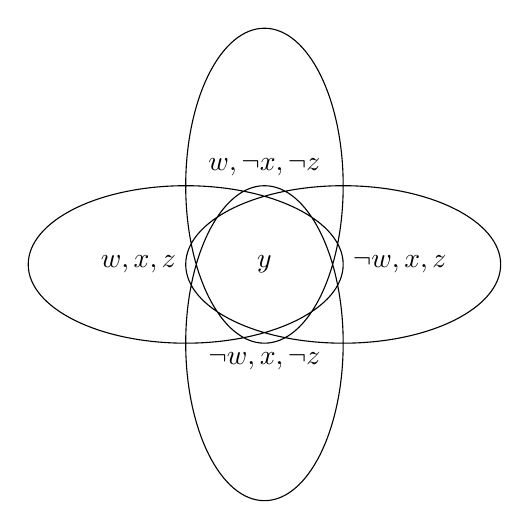
\begin{tikzpicture}
        \draw[] (-1,0) ellipse (2 and 1) node[anchor=east]{$w, x, z$}
                (0,1) ellipse (1 and 2) node[anchor=south]{$w, \neg x, \neg z$}
                (1,0) ellipse (2 and 1) node[anchor=west]{$\neg w, x, z$}
                (0,-1) ellipse (1 and 2) node[anchor=north]{$\neg w, x, \neg z$};
        \node (0,0) {$y$};
    \end{tikzpicture}
    \caption{Visualisation of a flower with 4 petals and $H = \{y\}$.}
    \label{fig:flower}
\end{figure}

\subsection{Algorithm}
% Describe the recursive algorithm
The Sparsification Algorithm at each step finds the best flower and then adds
the petals to one copy of the formula and the heart to the other copy of the formula,
removing redundant clauses. The algorithm then applies itself recursively to the two
new formulas. If there are no good flowers, then we are done. This algorithm can
be seen in Algorithm \ref{alg:sparse}.

\begin{algorithm}
\caption{Sparsification Algorithm (\texttt{sparsify})}
\label{alg:sparse}
\vspace{5pt}
\KwIn{$k$-CNF Formula $F$, $k \in \mathbb{N}$, $\epsilon > 0$}
\KwOut{$F'_1, F'_2, \dots, F'_t$}
\hrulefill\\

\nl $G = \{C_1, C_2, \dots C_s\} \gets \texttt{best\_flower}(F, \epsilon, k)$ \\
\nl \If{$F$ contains a good flower}{
    \nl $H \gets \bigcap_{C \in G}C$ \\
    \nl $P \gets \{C \setminus H : C \in G\}$ \\
    \nl $F_{\textit{heart}} \gets \texttt{reduce}(F \cup \{H\})$ \\
    \nl $F_{\textit{petals}} \gets \texttt{reduce}(F \cup P)$ \\
    \nl \Return{ }$\texttt{sparsify}(F_{\textit{heart}}, k, \epsilon) \cup$ \\ 
    $\hspace{30pt} \texttt{sparsify}(F_{\textit{petals}}, k, \epsilon)$ \\
}
\nl \Else{
    \nl \Return{$F$}
}
\end{algorithm}

\begin{figure}
    \centering
    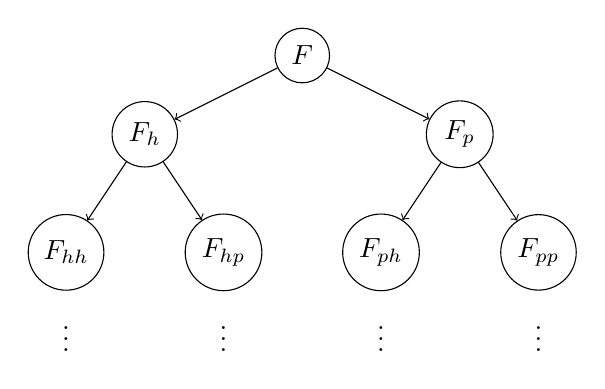
\begin{tikzpicture}
        \node[draw, circle] (A) at (0,0)     {$F$};
        \node[draw, circle] (B) at (-2,-1)   {$F_h$};
        \node[draw, circle] (C) at (2,-1)    {$F_p$};
        \node[draw, circle] (D) at (-3,-2.5) {$F_{hh}$};
        \node[draw, circle] (E) at (-1,-2.5) {$F_{hp}$};
        \node[draw, circle] (F) at (1,-2.5)  {$F_{ph}$};
        \node[draw, circle] (G) at (3,-2.5)  {$F_{pp}$};
        
        \node (H) at (-3, -3.5) {\vdots};
        \node (H) at (-1, -3.5) {\vdots};
        \node (H) at (1, -3.5) {\vdots};
        \node (H) at (3, -3.5) {\vdots};
        
        \path[->]   (A) edge (B);
        \path[->]   (A) edge (C);
        \path[->]   (B) edge (D);
        \path[->]   (B) edge (E);
        \path[->]   (C) edge (F);
        \path[->]   (C) edge (G);
    \end{tikzpicture}
    \caption{Visualisation of the first two recursive levels of Algorithm \ref{alg:sparse}}
    \label{fig:tree}
\end{figure}

A clause $D \in F$ is considered redundant if there is a clause $C \in F$ such that $C \subseteq D$.
Clause $D$ can be removed from $F$ without changing the satisfiability of $F$. This is because
satisfying $C$ automatically satisfies $D$, hence $D$ has no effect on the satisfiabilty of $F$.
The algorithm for removal of redundant clauses can be seen in Algorithm \ref{alg:reduce}.

\begin{algorithm}
\caption{Formula Reduction (\texttt{reduce})}
\label{alg:reduce}
\vspace{5pt}
\KwIn{$F$ a formula}
\KwOut{$F'$ a formula equivalent to $F$ with redundant clauses removed}
\hrulefill\\

\nl \For{$C, D \in F^2$}{
    \nl \If{$C \subseteq D$}{
        \nl $F \gets F \setminus D$ \\
    }
}
\nl \Return{$F$}
\end{algorithm}

To find the best flower we can take advantage of the fact that the largest possible heart will
at most be of size $k$. So we don't need to consider every subset of the clauses in $F$, but
just all all possible hearts which is polynomial in $n$. This algorithm can be seen in Algorithm \ref{alg:best_flower}, and
it runs in time $\mathcal{O}(k^3(2n)^{k}m\log k)$. Since $k$ is a constant then this is $\mathcal{O}(n^{k}m)$, which even when
$m = poly(n)$ is still polynomial in $n$. Correctness of Algorithm \ref{alg:best_flower} follows from the application of the
definition of a good flower from Equation \ref{eq:good_flower}, and from the fact that flowers are considered in
order from best to worst, so the best flower will always be returned if one exists.

\begin{algorithm}
\caption{Finding the best flower (\texttt{best\_flower})}
\label{alg:best_flower}
\vspace{5pt}
\KwIn{$k$-CNF formula $F$, $k \in \mathbb{N}, \epsilon > 0$}
\KwOut{$G = \{C_1, C_2, \dots, C_s\}$, the best flower good flower in $F$ if any}
\hrulefill\\

\nl \For{$l \in \{1, 2, \dots, k\}$}{
    \nl \For{\text{heart\_size} $\in \{k, k-1, \dots, 1\}$}{
        \nl $F^{\ast} \gets \{C \in F: |C| = l\}$ \\
        \nl \For{$H \in \{H \subseteq F^* : |H| = \text{heart\_size}\}$}{
            \nl $G \gets \emptyset$ \\
            \nl \For{$C \in F^{\ast}$}{
                \nl \If{$H \subseteq C$}{
                    \nl $G \gets G \cup C$ \\
                }
            }
            \nl \If{$|G| \geq \theta_{l - \text{heart\_size}}$}{
                \nl \Return{$G$} \\
            }
        }
    }
}
\nl \Return{\text{$F$ contains no good flower}} \\
\end{algorithm}

\section{Execution of Algorithms}
To better understand Algorithm \ref{alg:sparse} it can be helpful to go through a simple example.
We will start with a small CNF formula that we want to sparsify. We let $k = 3$, $n=3$, we let $\epsilon$ be sufficiently large
so that the sequence of $\theta$s become small enough for any flower with at last 2 petals to be good.
The example CNF formula is given as follows.
\begin{align*}
    F = &(\neg x_{1} \lor \neg x_{3} \lor x_{2}) \land (\neg x_{1} \lor \neg x_{2} \lor x_{2}) \land \\
    &(\neg x_{1} \lor x_{3} \lor x_{1}) \land (\neg x_{1} \lor \neg x_{2} \lor x_{1}) \land\\
    &(\neg x_{3} \lor x_{2} \lor x_{1})\\
\end{align*}
Notice that the literals $\neg x_1$ and $\neg x_2$ appears in 2 clauses in $F$, this becomes the heart of the first flower.
The two subformulas obtained after applying Algorithm \ref{alg:reduce} are given as follows where $h$ denotes the
subformula resulting from adding the heart of the first flower and $p$ denotes the subformula resulting from adding
the petals.
\begin{align*}
    h : &(\neg x_{1} \lor \neg x_{3} \lor x_{2}) \land (\neg x_{3} \lor x_{2} \lor x_{1}) \land\\
    &(\neg x_{1} \lor \neg x_{2}) \land (\neg x_{1} \lor x_{3} \lor x_{1})\\
    p : &(x_{2}) \land (x_{1})\\
\end{align*}
The subformula resulting from adding the heart still has a good flower with $(\neg x_3 \lor x_2)$ as the heart,
so the algorithm does not terminate.
\begin{align*}
    hh : &(\neg x_{1} \lor \neg x_{2}) \land (\neg x_{1} \lor x_{3} \lor x_{1})\land (\neg x_{3} \lor x_{2})\\
    hp : &(x_{1}) \land (\neg x_{1})\\
\end{align*}
No more flowers can be formed at this point, so the algorithm terminates. Note that not every subformula is satisfiable,
namely $hp$, but as long as $F$ is satisfiable the disjunction of all the subformulas is satisfiable.
In this case the subformula formed at the first petal branch $p$ is satisfiable and
yields a satisfying assignment to $F$.


\section{Proof}
\subsection{Satisfiability of \texorpdfstring{$F$}{Formula}}
To prove point 1 from Corollary \ref{cor:ksat_sparse}
we shall aim to show that $F$ is satisfiable if and only if $\bigvee_{i}^{t}F'_i$ is satisfiable.
\begin{proof}
    Consider a non-leaf node in the tree of recursive calls, pictured in Figure \ref{fig:tree}, let
    the formula at this point be $F^{\ast}$. since this is an non-leaf node, then it has a good
    flower $G$ and two children $F_h^{\ast}$ and $F_p^{\ast}$ for the heart branch and petal branch respectively.
    If either $F_h^{\ast}$ or $F_p^{\ast}$ is satisfiable then either the heart or all of the petals of $G$
    are satisfiable. This means that all clauses in $G$ are satisfiable and any clauses that were made
    redundant in $F_h^{\ast}$ or $F_p^{\ast}$ will also be satisfiable in $F^{\ast}$. All other clauses
    remain the same between $F_h^{\ast}$ or $F_p^{\ast}$ and $F^{\ast}$. Hence these clauses must also be
    satisfiable. Thus we have that $F^{\ast}$ is satisfiable if $F_h^{\ast}$ or $F_p^{\ast}$ is satisfiable.
    Since our choice of $F^{\ast}$ was arbitrary, this holds of all non-leaf nodes. Therefore, via induction, we have that if
    $\bigvee_{i}^{t}F'_i$ is satisfiable then $F$ is satisfiable.
    
    To see the converse, let $F$ be satisfiable and let $\alpha$ be the satisfying assignment.
    If $F$ is not also a leaf node then it has a good flower $G$.
    Notice that for a flower $G \subseteq F$, $\alpha$ must either satisfy the heart of the flower
    or all of the petals. So either $F_h$ or $F_p$ must be satisfied. By repeated application of this argument on $F_h$ and $F_p$
    we find that at least one of the leaves must be satisfiable. Which is what we require.
\end{proof}

The proof of point 2 that the algorithm does not add any new variables is obvious from looking at
Algorithm \ref{alg:sparse}.

\subsection{Formulas are linear in \texorpdfstring{$n$}{n} when the algorithm terminates}

\begin{definition}
    Given a CNF formula $F$, a literal $u$ and an integer $l \in \mathbb{N}$, let
    \begin{align}
        d_l(u, F) &= |\{C \in F : |C| = l \land u \in C\}| \label{eq:largest_flower_u} \\
        d_l(F) &= \max_u \{d_l(u, F)\} \label{eq:largest_flower}
    \end{align}
\end{definition}

We can interpret the first function as the size of the largest flower with clauses of size $l$
and with $u$ in the heart. Note that the flowers do not need to be good.
The second function can therefore be interpreted as the largest
flower with clauses of size $l$. This leads to the first observation.
% no good flower --> d_l(f) <= theta_l-1 - 1

\begin{lemma} \label{lem:no_good}
    Let $F$ be a ($\leq k$)-CNF formula that contains no good flowers with clauses of size $l$,
    then $d_l(F) \leq \theta_{l-1} - 1$.
\end{lemma}
\begin{proof}
    Suppose that $d_l(F) \geq \theta_{l-1}$. From the definition of $d_l(F)$ 
    in Equation \ref{eq:largest_flower}, this means that
    \begin{equation} \label{eq:many_petals}
        \exists u : |\{C \in F : |C| = l \land u \in C\}| \geq \theta_{l-1}
    \end{equation}
    Consider the flower $G$ of clauses with length $l$ with $u \in H$.
    We know that from Equation \ref{eq:many_petals} this flower has $\theta_{l-1}$ petals,
    however, since the heart is at least of size 1 then the length of the petals is $\leq l-1$.
    Therefore, from equation \ref{eq:good_flower} the flower $G$ is good.
    Thus
    \begin{equation} \label{eq:impl_no_flower}
        d_l(F) \geq \theta_{l-1} \implies F \text{ has a good flower of size $l$}
    \end{equation}
    Therefore, if we take the contrapositive of (\ref{eq:impl_no_flower}) we obtain what we want to show.
    \begin{equation}
        F \text{ does not have a good flower of size $l$}
        \implies d_l(F) \leq \theta_{l-1} - 1
    \end{equation}
\end{proof}
% corollary that |F| is O(n)
\begin{corollary} \label{cor:no_good}
    Let $F$ be a ($\leq k$)-CNF formula without any good flowers.
    Then $|F| \leq 2k\theta_{k-1} \cdot |vars(F)|$.
\end{corollary}
\begin{proof}
    We can apply lemma \ref{lem:no_good} for all clause lengths.
    Thus, 
    \begin{align}
        \forall l \in \{1,2,\dots,k\}:& \quad d_l(F) \leq \theta_{l - 1} - 1 \\
        \forall l \in \{1,2,\dots,k\}:& \quad \forall u \in lits(F): d_l(u, F) \leq \theta_{l-1}-1
    \end{align}
    Since there are at most $2 \cdot |vars(F)|$ literals in $F$, summing over $u$ yields
    \begin{equation}
        \forall l \in \{1,2,\dots,k\}: \sum_{u \in lits(F)} d_l(u, F) \leq 2\theta_{l-1}\cdot |vars(F)| \\
    \end{equation}
    Additionally, since every clause contains at least one literal then 
    $|\{C \in F : |C| = l\}| \leq \sum_{u \in lits(F)} d_l(u, F)$ since if $u \in C$ then $C$ contributes to $d_l(u, F)$.
    Therefore
    \begin{equation} \label{eq:clauses_size_l}
        \forall l \in \{1,2,\dots,k\}: |\{C \in F : |C| = l\}| \leq 2(\theta_{l-1} - 1) \cdot |vars(F)| \\
    \end{equation}
    Then we can sum up across all $l$ to get
    \begin{equation}
        |F| \leq 2 \sum_{l=1}^{k}(\theta_{l-1} - 1) \cdot |vars(F)|
    \end{equation}
    Recall that $\theta_i > \theta_{i-1}$, so we can upper bound all $\theta_{l-1}$ by $\theta_{k-1}$.
    \begin{align}
        |F| \leq& 2 \sum_{l=1}^{k}(\theta_{k-1} - 1) \cdot |vars(F)| \\
        |F| \leq& 2k\theta_{k-1} \cdot |vars(F)|
    \end{align}
\end{proof}

Observe that $2k\theta_{k-1}$ is a constant that is independent of $n$, hence we satisfy point 3)
from Corollary \ref{cor:ksat_sparse} of the Sparsification Lemma by setting $c(k,\epsilon) = 2k\theta_{k-1}$.

\subsection{There are subexponentially many leaves}

The final point is to show that $t \leq 2^{\epsilon n}$. This is 
the most involved section of the proof. We will show two things, which
will uppert bound the number of leaves in the recursion tree. Firstly, we will
claim that the longest path from the root to any leaf is at most $\alpha \cdot n$,
for some constant $\alpha \in \mathbb{N}$
Secondly, we will show that the number of branches that correspond to adding
petals to the formula is low. Specifically, we will show that the number of 
petal branches is at most $\frac{kn}{\delta}$. The constants $\alpha$ and $\delta$ will depend only
on the choices of of $k$ and $\epsilon$.

To get a sense for the number of leaves in the recursion tree, consider that
each path from the root to a leaf can be written as a sequence of p's and h's,
with p's corresponding to when the recursion tree branched to add petals and h's
corresponding to the when the recursion tree branched to add the heart of the flower.
The start of this recursion tree can be seen in Figure \ref{fig:tree}. The four
nodes at the bottom show the start of this sequence of p's and h's.
To then count the number of leaves in the recursion tree, we need to just count
the number of sequences. This can be done by summing the number of permutations
of p's and h's for each number of petal branches. The number of
paths from the root to a leaf with exactly $P$ petal branches would be given
by $\binom{\alpha \cdot n}{P}$. So therefore, if we know that there are
at most $\frac{kn}{\delta}$ petal branches then the total number of leaves is given by
\begin{equation} \label{eq:num_leaves_idea}
    \sum_{i}^{kn / \delta} \binom{\alpha \cdot n}{i} \leq 2^{H(\frac{k}{\alpha \cdot \delta}) \alpha n}
\end{equation}
where $H(x) = -x \log(x) - (1-x)\log(1-x)$ is the binary entropy function. This bound
can be obtained from Stirling's approximation of $n!$ (for more details see \cite{flum2006parameterized}).
We will show that $H(k / \alpha \delta) \alpha \leq \epsilon$ which would complete the proof.
% after added clauses of size j, level j remains sparse

\begin{lemma} \label{lem:rem_sparse}
    Let $F$ be the current formula at a non-leaf node occurring in the recursion tree
    as exemplified in Figure \ref{fig:tree}. Let $G = \{C_1, C_2, \dots, C_s\}$ be the flower
    identified as the best flower at this node. Denote $F'$ as a child of $F$ in the recursion
    tree. If $|C_i| = l$, then $F'$ would be formed by adding clauses of size $1 \leq j < l$ to $F$.
    We claim that
    \begin{equation}
        d_j(F') \leq 2 \cdot \theta_{j-1}
    \end{equation}
\end{lemma}
\begin{proof}
    There are two cases that need to be considered. The first is when 
    $F' = \texttt{reduce}(F \cup \bigcap_{C \in G} C)$, i.e. by adding the heart of
    the flower to $F$ and removing redundant clauses. The second is when
    $F' = \texttt{reduce}(F \cup \{C \setminus H : C \in G\})$ where $H$ is the heart of the flower,
    i.e. adding all the petals to $F$ and removing redundant clauses.
    \subsubsection{Case: Adding the heart to $F$}
    Recall that a flower is considered better than another if has shorter clauses. Therefore, since
    the best flower is picked at every step, there cannot have been a good flower in $F$ with
    clauses all of size $j$, since $j < l$. Then from Lemma \ref{lem:no_good}, we can say that
    \begin{equation}
        d_j(F) \leq \theta_{j-1} - 1
    \end{equation}
    Then, since only one clauses is added to $F'$, namely the heart and
    this is a clause of size $j$ so then we can conclude that
    \begin{equation}
        d_j(F') \leq \theta_{j-1} \leq 2 \cdot \theta_{j - 1}
    \end{equation}
    which is what we require.
    \subsubsection{Case: Adding petals to $F$}
    For the sake of contradiction, we will assume that $d_j(F') \geq 2 \cdot \theta_{j-1} + 1$.
    Recall, from the definition of $d_j(F)$ in Equation \ref{eq:largest_flower}, this means that there exists some literal
    $u$ that appears in $\geq 2 \cdot \theta_{j-1} + 1$ clauses of size $j$ in $F'$. Since
    we know that there was no good flower with clauses of size $j$ in $F$ then we know
    from Lemma \ref{lem:no_good}, that $d_j(u, F) \leq \theta_{j-1} - 1$. So then, since
    there are $\geq 2 \cdot \theta_{j-1} + 1$ clauses of size $j$ containing a literal $u$ in $F'$
    but only $\leq \theta_{j-1} - 1$ in $F$, then these clauses must have been added to $F'$
    from the petals of the flower, i.e. $d_j(u, \{C_1 \setminus H, C_2 \setminus H, \dots, C_t \setminus H\}) \geq \theta_{j-1}$ where $H$ is the heart of the flower. However, we can form a better flower in $F$ with $\{u\} \cup H$
    as the heart. This is a good flower because the new petals have
    size $j-1$ and we know that there are more than $\theta_{j-1}$ of them,
    so it satisfies Equation \ref{eq:good_flower} and
    is a good flower. This is a contradiction since the heart is larger and hence it is a better flower than
    the one picket in $F$, but Algorithm \ref{alg:best_flower} always picks the best flower.
    We then have that our assumption must be false and
    \begin{equation}
        d_j(F') \leq 2 \cdot \theta_{j - 1}
    \end{equation}
    as required. This concludes the proof.
\end{proof}
The interpretation of this proof is that once a clause of size $j$ is added to a formula
in the recursion tree, then the number of clauses of size $j$ will be linear in $n$. This is because
adding clauses of a different size cannot increase the number of clauses of size $j$, and
adding clauses of size $j$ invokes the lemma to show that this level is still linear in $n$.

We introduce the notion of \textit{Native} and \textit{Immigrant} clauses, meaning clauses
that were in the original formula $F$ at the root of the recursion tree
and clauses that were added as hearts and petals respectively.
Note that only \textit{Immigrants} can cause a clause to be removed from a formula in a call to
\texttt{reduce}.

We will now bound the number of \textit{Immigrant} clauses that can be removed by a single clause
in a call to \texttt{reduce}.
\begin{lemma} \label{lem:max_remove}
    For a formula $F$, in a call to \texttt{reduce($F$)}, a single clause $C$ can remove at most
    $2 \cdot \theta_{j - 1}$ \textit{Immigrant} clauses of size $j$ in $F$
\end{lemma}
\begin{proof}
    If no \textit{Immigrant} clauses of size $j$ exist in $F$ then none can be removed and we are done.
    Otherwise, since a clause of size $j$ has at some point been added to $F$
    we can apply Lemma \ref{lem:rem_sparse} to say that $d_j(u, F) \leq 2 \cdot \theta_{j - 1}$,
    where $u$ is a literal contained in the clause $C$. It then follows that $C$ can be a
    subset of at most $2 \cdot \theta_{j-1}$ clauses of size $j$. Since these are the clauses that
    are removed by $C$, then we are done.
\end{proof}

We will now attempt to bound the number of \textit{Immigrant} clauses added to the formula
along a path from the root to the leaf. To do this, we define a sequence of numbers
$\gamma_1 = 2$ and $\gamma_l = 4 \theta_{l - 1}\gamma_{l-1}$.
\begin{lemma} \label{lem:bound_immigrants}
    For a path from the root to a leaf in the recursion tree and for $1 \leq l \leq k - 1$,
    let $I_{\leq l}$ denote the number of \textit{Immigrant} clauses of size $\leq l$ that are added along the
    path. Then
    \begin{equation}
        I_{\leq l} \leq \gamma_l \cdot n
    \end{equation}
\end{lemma}
% \begin{proof}
%     Let $F$ denote the formula at the root of the recursion tree, let $F'$ denote the formula
%     at the leaf and let $R_l$ be the number of \textit{Immigrant} clauses of size $l$ that are removed
%     along the path from $F$ to $F'$.
%     
%     Notice that an \textit{Immigrant} clause of size $l$ is either removed by some other \textit{Immigrant}
%     clause of size $\leq l - 1$ or is still in $F'$ at the end. It therefore follows that
%     \begin{equation*}
%         I_l \leq R_l + \textit{\#number of clauses of size $l$ in $F'$}
%     \end{equation*}
%     From Equation \ref{eq:clauses_size_l} in Corollary \ref{cor:no_good} we know that \#number of clauses of size $l$ in $F'$ is at most
%     $2 \cdot \theta_{l-1} n$. We will consider induction on $l$. Suppose that a clause $D$ of size $l$
%     was removed in the \texttt{reduce} step, this means that an \textit{Immigrant} clause $C$ with
%     $C \subseteq D$ was added to the formula. By Lemma \ref{lem:max_remove}, we know that this
%     clause could have removed at most $2 \cdot \theta_{l-1}$ of size $l$. By the inductive hypothesis,
%     the algorithm adds at most $\gamma_{l-1} n$ clauses of size $\leq l-1$
%     along the path from the root to the leaf. In total these clauses can then remove at most
%     $2 \theta_{l-1}\gamma_{l-1}n$ \textit{Immigrant} clauses of size $l$.
%     \begin{equation}
%         R_l \leq 2 \theta_{l-1}\gamma_{l-1}n
%     \end{equation} % Question why the hell we can go from removing clauses of size l -1 to removing all clauses of size l
%     % it's simply a bound and \theta_{l-1} is greater than all the smaller thetas, so the bound holds
%     Combining bounds for $R_l$ and for the \# number of clauses of size $l$ in $F'$ we get
%     \begin{equation}
%         I_l \leq 2 \theta_{l-1}\gamma_{l-1}n + 2 \theta_{l-1}n \leq 4 \theta_{l-1}\gamma_{l-1}n = \gamma_{l}n
%     \end{equation}
%     The last step follows from our definition of $\gamma_l$. What remains is to show the inductive base,
%     this follows from the fact that a clause is never added twice, so therefore $I_1$ could at most be
%     the number of variables in $F'$ and since there are no more variables in $F'$ than in $F$ we can
%     conclude that $I_1 \leq n = \gamma_1 n$. This concludes the proof.
% \end{proof}
\begin{proof}
    We will show this by induction on $l$.
    Let $F$ denote the formula at the root of the recursion tree and let $F'$ denote the formula
    at a leaf. Let $R_l$ be the number of \textit{Immigrant} clauses of size exactly $l$ that are
    removed along the path from $F$ to $F'$
    
    The base case where $l = 1$ follows from the fact that there are only $2n$ clauses of size 1,
    so $I_{\leq l} \leq 2n = \gamma_1 n$. We assume that our inductive hypothesis holds for $l - 1$.
    \begin{equation} \label{eq:inductive_hyp}
        I_{\leq l - 1} \leq \gamma_{l-1} n
    \end{equation}
    We now show that this implies that the lemma holds for $l$.
    
    Denote $I_l$ as the number of \textit{Immigrant} clauses of size exactly $l$ that are added along
    the path from $F$ to $F'$. Each such added clause will either be removed at some point in the path
    or remain in $F'$. Hence we can bound $I_l$ from above.
    \begin{equation} \label{eq:bound_immigrant_exact}
        I_l \leq R_l + |\{C \in F' : |C| = l\}|
    \end{equation}
    From Equation \ref{eq:clauses_size_l} in Corollary \ref{cor:no_good} we know that
    $|\{C \in F' : |C| = l\}| \leq 2 \theta_{l-1}n$.
    
    We will now bound $R_l$. If $R_l \neq 0$ then there is some clause $D$ of size $l$ that was removed
    by some \textit{Immigrant} clause $C \subset D$ where $|C| \leq l -1$. 
    By Lemma \ref{lem:max_remove} we know that this clause
    could have removed at most $2 \theta_{l-1}$ clauses of size $l$. From the inductive hypothesis
    we know that there are at most $\gamma_{l-1} n$ such clauses. Hence we obtain the following bound on $R_l$.
    \begin{equation} \label{eq:bound_removals}
        R_l \leq 2\theta_{l-1}\gamma_{l-1}n
    \end{equation}
    Additionally, we observe that
    \begin{equation} \label{eq:ineq_eq}
        I_{\leq l} = I_{\leq l - 1} + I_{l}
    \end{equation}
    
    Combining these inequalities we obtain the following:
    \begin{align*}
        I_{\leq l} &= I_{\leq l - 1} + I_{l} \\
        &\leq \gamma_{l-1}n + R_l + |\{C \in F' : |C| = l\}| \\
        &\leq \gamma_{l-1}n + 2\theta_{l-1}\gamma_{l-1}n + 2 \theta_{l-1}n \\
        &\leq 4\theta_{l-1}\gamma_{l-1}n \\
        &\leq \gamma_{l}n
    \end{align*}
    By the principle of induction we know that this holds for all $l \geq 1$, which concludes the proof.
\end{proof}

Additionally, since at every step in the recursion, at least one \textit{Immigrant} clause is added
to the formula and this clause must have size $\leq k - 1$ then it immediately follows that
\begin{corollary}
    Any path from root to leaf has at most $\gamma_{k-1} n$ edges.
\end{corollary}

Since the length of a path from the root to a leaf is at most $\gamma_{k-1}n$,
if we set $\alpha = \gamma_{k} \geq \gamma_{k-1}$ then we achieve our first goal of bounding the length of the longest
path by $\alpha \cdot n$. What remains is to show that the number of petal branches in the recursion tree
is at most $\frac{kn}{\delta}$.

\begin{lemma} \label{lem:bound_petals}
    For any path from the root to a leaf in the recursion tree, at most $\frac{kn}{\delta}$ branches
    are from adding petals.
\end{lemma}
\begin{proof}
    For a fixed path from the root to a leaf in the recursion tree, let $P_l$ be the number of times 
    that petals are added to the formula with petals of size $l$.
    Recall the definition of a good flower,
    Equation \ref{eq:good_flower} tells us that such a flower must have had at least $\theta_{l}$
    petals. Therefore, we can conclude that along this path $P_l \cdot \theta_l$ individual petal
    clauses of size $l$ would have been added. Recall from Lemma \ref{lem:bound_immigrants} that
    $I_{\leq l}$ is the number of immigrant clauses of size $\leq l$ added along a path. Since every petal
    clause is an immigrant we obtain
    \begin{equation}
        I_{\leq l} \geq P_l \cdot \theta_l
    \end{equation}
    However, from Lemma \ref{lem:bound_immigrants} we also have that $I_{\leq l} \leq \gamma_l n$, so
    \begin{align*}
        P_l \cdot \theta_l \leq &I_{\leq l} \leq \gamma_l n \\
        P_l \cdot \theta_l &\leq \gamma_l n \\
        P_l &\leq \frac{\gamma_l}{\theta_l}n
    \end{align*}
    Thus, if we were to have that $\delta = \frac{\theta_l}{\gamma_l}$ then we obtain that $P_l \leq \frac{n}{\delta}$.
    If we sum over all $l$ to get the total number of petal branches then we obtain what we require.
    \begin{align*}
        \text{\#petal branches} &= \sum_{l=1}^{k} P_l \\
        \text{\#petal branches} &\leq \sum_{l=1}^{k} \frac{n}{\delta} \\
        \text{\#petal branches} &\leq \frac{kn}{\delta}
    \end{align*}
    This concludes the proof.
\end{proof}

We are now ready to set the constants $\theta_i$. We require that $\frac{\theta_l}{\gamma_l} = \delta$
from Lemma \ref{lem:bound_petals}
and that $\gamma_l = 4\gamma_{l-1}\theta_{l-1}$ from Lemma \ref{lem:bound_immigrants}.
Consider $\gamma_{l} = (4\delta)^{2^{l-1}-1}$ and $\theta_{l} = \delta \gamma_l$. Check that we have $\frac{\theta_l}{\gamma_l} = \delta$
as required. We also check that
\begin{align*}
    \gamma_l &= 4 \gamma_{l-1} \theta_{l-1} \\
    &= 4 \delta \gamma_{l-1}^2 \\
    &= 4 \delta ((4\delta)^{2^{l-2}-1})^2 \\
    &= (4\delta)^{2^{l-1}-1}
\end{align*}
as required.

We have now bounded the length of the longest path in the recursion tree by $\gamma_k n$
and bounded the number of petal branches by $kn / \delta$.
We therefore have that the number of leaves in the recursion tree is bounded by
\begin{equation*}
    \sum_{i=0}^{kn / \delta} \binom{\gamma_k n}{i} \leq 2^{H(\frac{k}{\delta \gamma_k})\gamma_k n}
\end{equation*}

What remains is to show that $H(\frac{k}{\delta \gamma_k})\gamma_k \leq \epsilon$.
If we require that $\delta \geq k$ then we get that $\frac{k}{\delta \gamma_k} \leq \frac{1}{2}$.
Consider the binary entropy function
\begin{equation}
    H(x) = -x\log(x) - (1-x)\log(1-x)
\end{equation}
for small $x$ we have that $-x\log(x) \geq -(1-x)\log(1-x)$, so we can bound
\begin{equation}
    H(x) \leq -2x\log(x)
\end{equation}
Plugging in $x = k / (\delta \gamma_k)$, we obtain
\begin{align*}
    H(\frac{k}{\delta \gamma_k}) &\leq -2 \frac{k}{\delta \gamma_k} \log(\frac{k}{\delta \gamma_k}) \\
    &\leq -2 \frac{k}{\delta \gamma_k} (\log(k) - \log(\delta) - \log(\gamma_k)) \\
    &\leq -2 \frac{k}{\delta \gamma_k} (\log(k) - \log(\delta) - (2^{k-1} - 1)\log(4\delta)) \\
    &\leq -2 \frac{k}{\delta \gamma_k} (- 2^{k}\log(\delta)) \\
    &\leq 2 \frac{k2^{k}\log(\delta)}{\delta \gamma_k} \\
    H(\frac{k}{\delta \gamma_k})\gamma_k &\leq 2 \frac{k2^{k}\log(\delta)}{\delta}
\end{align*}
Therefore, given $k$ and $\epsilon$ all that remains is to choose our $\delta$ such that
\begin{equation}
    2 \frac{k2^{k}\log(\delta)}{\delta} \leq \epsilon
\end{equation}
Which is what we require for our claim that there are at most $2^{\epsilon n}$ leaves.
It immediately follows that the run time of the algorithm is $\mathcal{O}^{\ast}(2^{\epsilon n})$, since
there can be at most $2^{\epsilon n}$ recursive calls and each takes polynomial time.

This concludes the proof. So we can say that Equation \ref{eq:run_time} holds and if 3-SAT
can be solved in subexponential time, then so can $k$-SAT for all $k \geq 3$.
% bound on number of clauses entering (Any path has at most beta_k-1 n edges)
% along a path there are few petal steps
% Bound on the number of leaves using the binary entropy function

\section{Exploration of the Lemma}
To gain a better understanding of the relationship between the constants $k, \epsilon, \delta, \gamma_l$ and $\theta_l$
consider the following.
\begin{align*}
    2 \frac{k2^{k}\log(\delta)}{\delta} &\leq \epsilon \\
    \frac{\log \delta}{\delta} &\leq \frac{\epsilon}{k \cdot 2^{k+1}}
\end{align*}
Using the following upper bound $\frac{\log x}{x} \leq \frac{\log(x + 1)}{x} \leq \frac{1}{\sqrt{1 + x}}$ \cite{topsok2006some}.
We can therefore choose $\delta$ such that
\begin{align*}
    \frac{1}{\sqrt{1 + \delta}} &\leq \frac{\epsilon}{k \cdot 2^{k+1}} \\
    \delta &\geq \frac{k^2 \cdot 2^{2k+2}}{\epsilon^2} - 1
\end{align*}
We can then note that $\delta$ grows exponentially with $k$ and polynomially with $\frac{1}{\epsilon}$.
Thus from the definition of $\gamma_l$ and $\theta_l$, we can see that they grow roughly as $\delta^{2^{l}}$,
so therefore we can justify our original claim that $\theta_l \gg \theta_{l-1}$.
\begin{example}
    We can consider an example where we have a 3-CNF formula that we wish to sparsify, $k = 3$ and we choose
    $\epsilon = 10^{-2}$. We can see that this leads to
    \begin{equation*}
        \delta \geq \frac{3^2 \cdot 2^{2 \cdot 3 + 2}}{{(10^{-2})}^{2}} - 1 = 23\,039\,999
    \end{equation*}
    We can the calculate the terms of $\gamma_l$ and $\theta_l$.
    \begin{table}
        \centering
        \begin{tabular}{l c c}
        \toprule
             $l$ & $\theta_l$ & $\gamma_l$ \\
             \midrule
             1 & 23\,039\,999 & 1  \\
             2 & $\sim 2.123 \cdot 10^{15}$ & 92159996 \\
             3 & $\sim 1.803 \cdot 10^{30}$ & $\sim 7.828 \cdot 10^{23}$ \\
        \bottomrule
        \end{tabular}
        \caption{Growth of Coefficients}
        \label{tab:coeffs_example}
    \end{table}
    The growth of these coefficients for this example can be seen in Table \ref{tab:coeffs_example}.
    Notice, that even for small examples these constants exhibit rapid growth. Therefore, even
    though we know from Corollary \ref{cor:no_good} that at the end of Algorithm \ref{alg:sparse},
    $|F| \leq 2k \cdot \theta_{k-1} n$ which is $\mathcal{O}(n)$, the constant hidden in the Big-$\mathcal{O}$
    is typically significantly larger than most practical instances of SAT which have typically at most on the
    order of $10^6$ clauses \cite{SAT_Comp2017}.
\end{example}

Therefore, due to large constants, the sparsification lemma is not easy to apply to $k$-SAT solvers
in the hopes of achieving better practical performance as measured by wall time. However, it is sufficient
to show that Equation \ref{eq:run_time} holds.

However, one by notice that there exists many upper and lower bounds in this proof which may have better bounds,
leading to smaller constants. For example, in Corollary \ref{cor:no_good} we bounded the sequence $(\theta_1 + \theta_2 + \dots + \theta_{k-1})$
by $k \theta_{k-1}$. Although, due to the rapid growth of $\theta_l$, this is almost $k$ times greater.
Hence it is possible that there exists tighter bounds than ones shown in this chapter.

\subsubsection{Numerical Tests}
To gain a better understanding of how the sparsification lemma behaves we implemented
the algorithms presented in this chapter and ran them on randomly CNF formulas.
Taking inspiration from the problem presented in the introduction, we generate CNF
formulas where $m = n^2$. Each clause picks 3 literals at random with uniform probability
with the additional requirement that all clauses must be unique. We do not concern ourselves
with whether the formulas are satisfiable or not.
Some results from these tests can be seen in Figures \ref{fig:sparsification}, \ref{fig:num_subformulas}, \ref{fig:tree_height}.

\begin{figure}
    \centering
    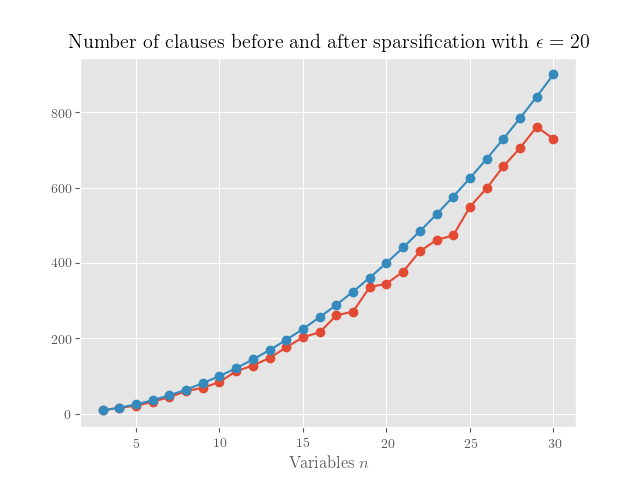
\includegraphics[scale=0.7]{Chapter4/Figs/sparsification_20.png}
    \caption{The size of the largest subformula compared with the size of the original formula}
    \label{fig:sparsification}
\end{figure}
\begin{figure}
    \centering
    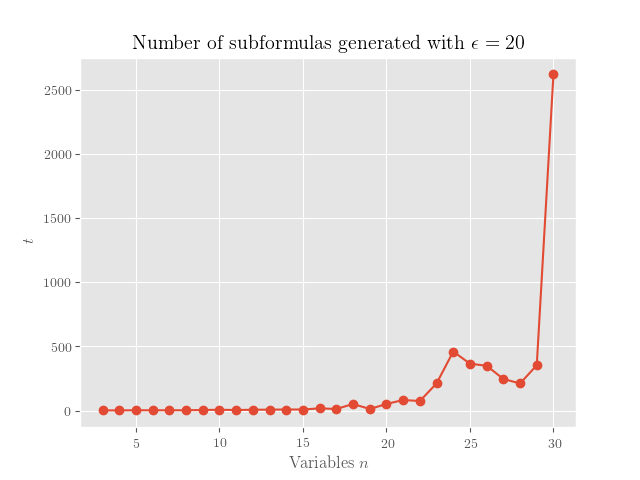
\includegraphics[scale=0.7]{Chapter4/Figs/subformulas_20.png}
    \caption{Number of subformulas returned}
    \label{fig:num_subformulas}
\end{figure}
\begin{figure}
    \centering
    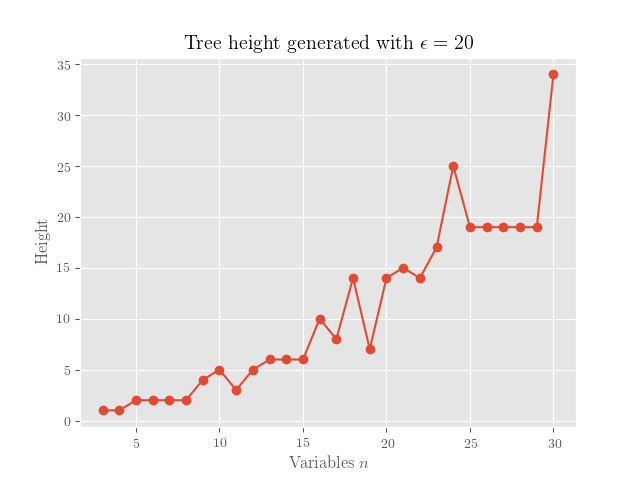
\includegraphics[scale=0.7]{Chapter4/Figs/tree_height_20.png}
    \caption{The height of the recursion tree for varying $n$}
    \label{fig:tree_height}
\end{figure}

As we can see in Figure \ref{fig:sparsification}, for small $n$ the largest subformula
is only slightly smaller than the size of the original formula. However, we note that
the bound for this instance was approximately $600n$, so for small $n$ the algorithm
could have done nothing whilst satisfying the bound. This suggests that often
Algorithm \ref{alg:sparse} will return CNF formulas sparser than required.

Due to computational restrictions, we were unable to test the behaviour of the algorithm
as the length of the original formula approaches that of the bound. We also note that
due to the large hidden constant in the bound on sparsity for small $n$ there are often
not enough unique clauses for the original formula to be above the bound on sparsity.

To get a sense for computational cost see Figures \ref{fig:num_subformulas} and \ref{fig:tree_height},
where we see rapid growth of the number of subformulas returned by Algorithm \ref{alg:sparse} and steady
growth in the height of the recursion tree. However, considering our choice of $\epsilon = 20$ we can
only guarantee that the number of subformulas returned is less than $2^{20n}$ which is a function growing much faster
than what we observe in Figure \ref{fig:num_subformulas}. This again suggests our theoretical bounds can be improved by
some constant factor.

Furthermore, even though Algorithm \ref{alg:best_flower} runs in polynomial time it quickly becomes infeasible
to the best flower of even the first formula. Considering that we let $m = n^2$ and $k=3$ the computational
complexity of Algorithm \ref{alg:best_flower} becomes $\mathcal{O}(n^5)$ where the hidden constant is $>100$.
While this is certainly polynomial time it makes it infeasible to test formulas large enough to be above
the bound on sparsity.

\subsubsection{Intuitions and Ideas for Further Work}
The sparsification lemma seems to capture an idea that dense formulas are somehow easy
since they can be made sparse in subexponential time potentially cutting away many clauses.
This is an idea that will be covered from another perspective in Chapter \ref{chap:structure}.
We can imagine that the hardest CNF formulas are those where $m$ is $\mathcal{O}(n)$, since
this can be enforced by the sparsification lemma, incurring only subexponential cost.

Furthermore, consider that the branching performed in Algorithm \ref{alg:sparse} is similar
to the branching performed by DPLL seen in Chapter \ref{chap:solvers}. However, in the worst case
DPLL runs in $\mathcal{O}(2^n)$. Impagliazzo et al. \cite{impagliazzo2001problems} comment
that branching on a disjunction of variables rather than single variables ends up requiring less
branching in total. This then brings up the question of whether the idea of branching on disjunctions
of variables could applied to SAT solvers. If we relax the requirement that the clause branched on
had to be the best flower and instead picked disjunctions of variables based on sensible heuristics that are efficiently computable,
would this lead to smaller recursion trees in algorithms based on DPLL? We leave this question for further work.
%!TEX root = ../thesis.tex
%*******************************************************************************
%****************************** Third Chapter **********************************
%*******************************************************************************
\chapter{Structures in SAT} \label{chap:structure}

% **************************** Define Graphics Path **************************
\ifpdf
    \graphicspath{{Chapter5/Figs/Raster/}{Chapter5/Figs/PDF/}{Chapter5/Figs/}}
\else
    \graphicspath{{Chapter5/Figs/Vector/}{Chapte5/Figs/}}
\fi

\section*{Introduction}
In this chapter we attempt to provide an explanation of why it is simultaneously
possible to have fast ``in practice'' SAT solving algorithms, as seen in Chapter
\ref{chap:solvers}, and also have standing conjectures about the complexity of
SAT that suggest that we should not expect to solve SAT in subexponential time,
as seen in Chapter \ref{chap:complexity}. From this it seems that many SAT instances
are significantly easier than their worst-case counterparts.

This discrepancy between the hardness of the worst-case instances and the typical
hardness has been known for NP-COMPLETE problems such as $k$-colouring \cite{turner1988almost}, where it was shown
by Turner et al. that ``almost all'' $k$-colourable
graphs could be coloured by a simple $\mathcal{O}(|V| + |E|\log k)$ time algorithm,
where ``almost all'' means that $\mathrm{Pr}[\text{Algorithm finds a colouring}] \to 1$
as $|V| \to \infty$. A similar argument could then be made for SAT via reduction to
$k$-colourability (see Figure \ref{fig:reduce_3col}).

We will cover exactly
where these hard worst-case instances lie by considering the clause ratio of an
instance and also considering a notion distance of an instance to a polynomial time tractable
sub-classes of SAT. We will also touch on the issue of attempting to determine whether
a single SAT instance is hard or not.

\section{Heavy-Tailed Distributions of Difficulty}
\subsection{Issues Measuring Expected Running Time of SAT Solvers}
A natural question when attempting to measure the difficulty of certain SAT instances
is whether in instance is inherently hard, or if the specific solver used was simply
unlucky with this instance.

To shed light on this issue Gomes et al. attempt to characterise
the distribution of run times for SAT solvers (with some random element)
on fixed SAT instances \cite{gomes2000heavy}. To do this they empirically measure
the number of backtrack steps required
to solve a SAT instance for a solver based on the Davis-Putnam-Logemann-Loveland procedure (DPLL)
\cite{davis1962machine}.
Gomes at al. demonstrate that the sample mean does not stabilise
with increasing the size of the sample.
This indicates that the distribution of backtracks required
has undefined moments, i.e has non-negligible tail probabilities.

This has the unfortunate consequence that a single SAT instance may appear
trivial to solve at one point and very challenging at another and there is no
well defined mean difficulty. This can be seen in Figure \ref{fig:erratic_mean}, which
shows a failure of the sample mean to converge to any value. Gomes et al. note
that the sample median, however, does converge quickly to a value of 1.

\begin{figure}[hb]
    \centering
    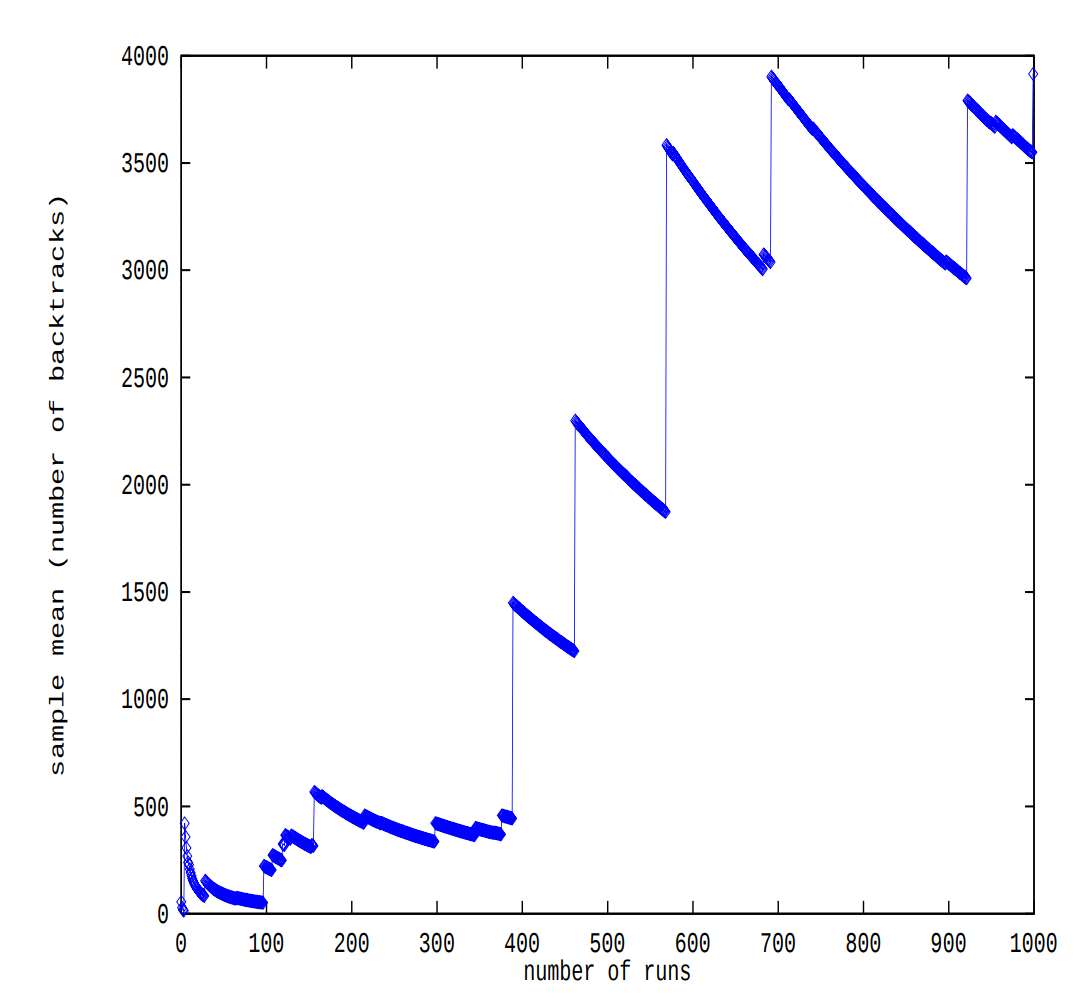
\includegraphics[scale=0.17]{sample_mean_backtracks.png}
    \caption[Sample mean of backtracks]{Sample mean of the number of backtracks required to solve a SAT encoding of the quasigroup completion problem.}
    \label{fig:erratic_mean}
\end{figure}



\subsection{Randomising SAT Solvers}
In order to permit a distribution over backtracks required,
a random element has to be added to the SAT solvers
being analysed. Gomes et al. consider modifications to Satz and Relsat
which are both based on DPLL. These
solvers use a collection of heuristics to determine which
variable to branch on. Gomes et al. define a constant $H$,
such that all variables that are in the top $H$-percent, as evaluated by
the heuristics, are chosen at random with
uniform probability.

\subsection{Pareto-L\'evy Distributions}
\subsubsection{Distributions with infinite moments}
Gomes et al. consider a class of distributions called Pareto-L\'evy distributions which have the following form.
\begin{align*}
    \text{P}(X > x) &\sim Cx^{-\alpha}, \hspace{5pt} x > 0 \footnotemark\\
    C &> 0\\
    0 < &\alpha < 2
\end{align*}
\footnotetext{Here $f(x) \sim g(x)$ is used to mean 
$\lim_{x \to \infty} \frac{f(x)}{g(x)} = 1$}
This means that the distribution decays polynomially in $x$ as opposed to exponentially, as would be the case
for a Gaussian distribution.
An example of a probability distribution with this form is the Cauchy distribution
which is defined as follows.
\begin{equation*}
    \text{Cauchy}(\gamma, \delta) = \frac{1}{\pi}\cdot\frac{\gamma}{\gamma^{2} + (x - \delta)^{2}}
\end{equation*}
For the Cauchy distribution $\alpha = 1$. For the Pareto-L\'evy distribution $\alpha = 0.5$.
\subsubsection{Distribution of Backtracks required by randomised SAT Solvers}
Gomes et al. empirically sample the number of backtracks required to solve a SAT instance for a
few different instances taken from different domains. These domains are the Quasigroup completion problem,
Scheduling, logistics planning and register allocation. For brevity only the scheduling example is shown here
in Figure \ref{fig:scheduling}. This plot shows the probability $\text{P}(X > x)$, where x is the number of backtracks required
to solve the instance on the randomised solver. The scale on the plot is logarithmic so a straight line
implies polynomial decay.
\begin{align*}
    m \cdot \log(x) + b &= \log(\text{P}(X > x))\\
    x^{m} e^{b} &= \text{P}(X > x)\\
    \text{P}(X > x) &\sim Cx^{m}
\end{align*}
Hence we can estimate $\alpha$ from the slope of the line in the plot.

\begin{figure}
    \centering
    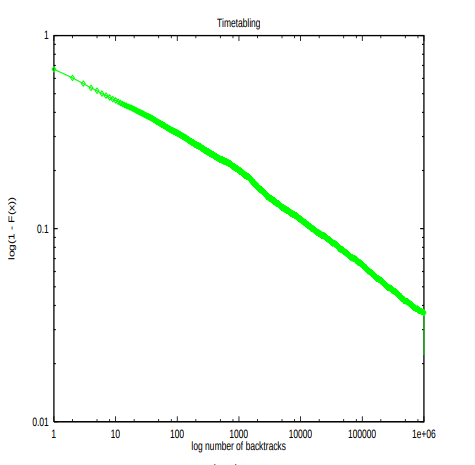
\includegraphics[scale=0.35]{scheduling_tails.png}
    \caption[Distribution of number of backtracks]{Cumulative $\log$ plot of the number of instances solved with a given number of backtracks. Gomes et al. estimates a value of $\alpha = 0.219$ for this problem}
    \label{fig:scheduling}
\end{figure}

\subsection{Motivation for rapid restarts in SAT solvers}
Gomes et al. go on to state that since there is non-negligible probability to the left
side of the distribution then a sequence of many short runs would be more effective than
a single long run. Gomes et al. then empirically validate their claim by modifying Satz and Relsat
to include rapid restarts when a certain number of backtracks is reached.
This results in an order of
magnitude reducing in the time to solve SAT instances,
although the point at which restarting is most
effective depended on the domain of the problem.

\subsection{Points of Caution}
From this we should be cautious to label any given SAT instance as difficult since
the underlying distribution of the number of backtracks required to find a satisfying
assignment has undefined mean and variance. As such we also cannot immediately trust a
sample of runs giving a mean runtime, since the mean does not converge to anything.
Ideally, we should consider the median runtime, which is defined for heavy-tailed distributions
and is therefor more trustworthy in empirical tests.

\section{Phase Transition}
Consider a SAT instance $F$ with few clauses compared to the number of variables,
intuitively this formula has many degrees of freedom and few constraints so
it is highly likely that $F$ will be satisfiable. Furthermore, if we consider
how a run of a backtracking solver would behave on such an instance, since it
only backtracks when it finds a conflict and few conflicts exist then it would
find an assignment without requiring many backtracking steps. If we instead
consider a SAT instance $F'$ with many clauses compared to the number of variables
we can see that a backtracking solver would be spending most of its time applying
unit propagation. Hence in this case also the solver would be able to decide
that $F'$ is not satisfiable quickly.

We call these instances underconstrained and overconstrained respectively.
Work by Cheeseman et al. suggests that all NP-COMPLETE problems have some
order parameter which exhibits a phase transition between underconstrained and 
overconstrained. Furthermore, the hard instances of an NP-COMPLETE problem
occur exactly at the point of the phase transition \cite{cheeseman1991really}.
Here, hardness is measured by the number of backtracking steps that are required
to solve an given instance of an NP-COMPLETE problem. Taking $k$-SAT as an example,
the order parameter is the ratio of the number of clauses to the number of variables
$\frac{m}{n}$ and the hardest instances of $k$-SAT are found at some critical value
$c_k$. This explains how Turner et al. were able to achieve their algorithm,
most random instances are far from the critical value \cite{turner1988almost}.

% ratios for ksat
\subsection{Transition Sharpness}
The phase transition is known to be ``sharp'' \cite{phase_transition}
in the following sense. Let
$U_k(n, m)$ be the uniform distribution over all $k$-CNF formulas with
$n$ variables and $m$ clauses and $c_k$ be the critical value, then
\begin{equation} \label{eq:sharp}
    \mathrm{Pr}_{F \sim U_k(n, m)}[F\text{ is satisfiable}] =
    \begin{cases}
        0 & \frac{m}{n} > c_k \\
        1 & \frac{m}{n} < c_k
    \end{cases}
    \quad\text{as }
    n \to \infty
\end{equation}
For 2-SAT this critical value is known to be $c_2 = 1$, \cite{chvatal1992mick, goerdt1996threshold}.
However, for all $k \geq 3$, no exact value of $c_k$ is known. Although it is known
that $3.003 < c_3 < 4.81$ and $c_3 \approx 4.24$ \cite{crawford1993experimental}
(see Figure \ref{fig:phase_sat_prob}).

\begin{figure}
    \centering
    \hspace{-2cm}
    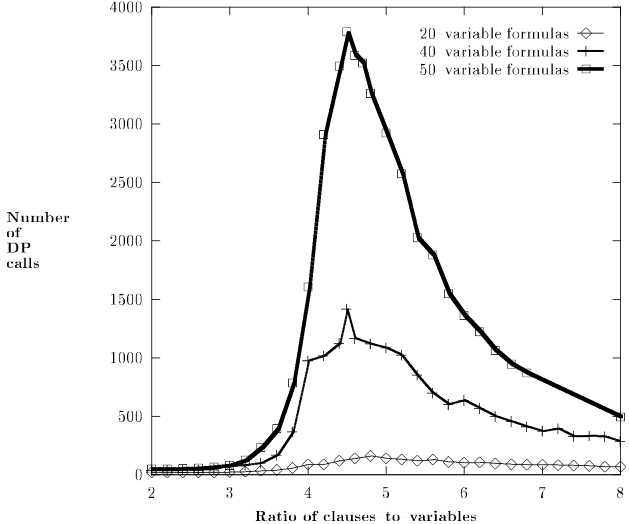
\includegraphics[scale=0.5]{DP_backtracks.png}
    \caption{Median number of backtracks required to solve a 3-SAT instance for varying
    clause ratio \cite{hard_and_easy_distributions}}
    \label{fig:phase_backtracks}
\end{figure}
\begin{figure}
    \centering
    \hspace{-2cm}
    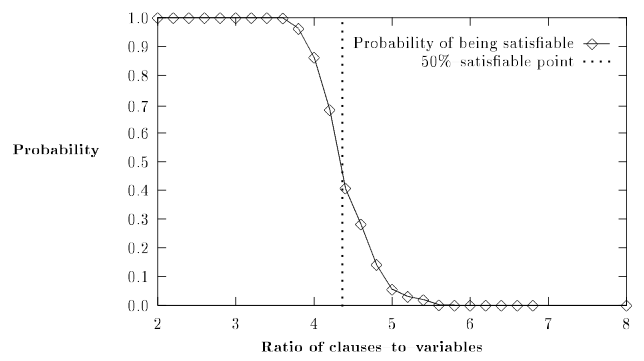
\includegraphics[scale=0.5]{phase_transition_probs.png}
    \caption{Probability that a random 3-SAT instance is satisfiable for varying
    clause ratio \cite{hard_and_easy_distributions}}
    \label{fig:phase_sat_prob}
\end{figure}

For large $n$ only instances close to critical values will be hard
(See Figure \ref{fig:phase_backtracks}).
This fact has been used by Mitchell et al. \cite{hard_and_easy_distributions}
to define probability distributions over $k$-SAT instances that are hard for
the purpose of creating new challenging benchmarks.

\subsubsection{Analogies to Spin Glasses and Statistical Mechanics}
Work by Kirkpatrick uses elements of statistical mechanics and an analogy of
random $k$-SAT to spin glasses to propose a form for phase transition.
Their work suggest that for some fundamental function $f$ and constants $c_k$
and $v$ then
\begin{equation}
    \mathrm{Pr}_{F \sim U_k(n, m)}[F \text{ is satisfiable}] = f\Big(\Big(\frac{m}{n} - c_k\Big) \cdot \frac{n^{1/v}}{c_k}\Big) % check this c_k substitution
\end{equation}
Using empirical methods $f$ and the constants $c_k$ and $v$ can be estimated.
Kirkpatrick et al. estimate $c_3 \approx 4.17$ and $v \approx 1.5$ \cite{kirkpatrick1994statistical}.
We note that this form for the satisfiability probability illustrates that
for any $\frac{m}{n} - c_k \neq 0$ then as $n \to \infty$ the probability tends
to $f(-\infty)$ or $f(\infty)$. If we
have that $\lim_{x \to -\infty}f(x) = 1$ and $\lim_{x \to \infty}f(x) = 0$ then we
can justify Equation \ref{eq:sharp}.


\subsection{Generalisations}
However, most ``in practice'' SAT instances do not have fixed clause length
and instead have many short and long clauses. Work by Gent et al. generalises
the SAT phase transition to mixed-clause instances \cite{phase_transition}.
Consider a probability distribution over the integers $\phi(k)$, let a $\phi$-SAT
formula $F$ be such that for a randomly selected clause $C \in F$
\begin{equation}
    \mathrm{Pr}[|C| = k] = \phi(k)
\end{equation}
i.e. clauses of size $k$ are picked to be in $F$ with probability $\phi(k)$.

Denote the critical value for a particular distribution $c_\phi$. Gent et al.
give a simple upper bound for $c_\phi$. Let $\alpha$ be an assignment chosen
uniformly at random and $C_k$ be an arbitrary clause of length $k$.
For a given distribution of clause lengths $\phi$ we define
$d_\phi$ as follows:
\begin{equation}
    d_\phi = \mathrm{Pr}_{k \sim \phi}[\alpha \text{ satisfies } C_k] = \sum_{k=1}^{\infty}\phi(k) \Big(1 - \Big(\frac{1}{2} \Big)^k \Big)
\end{equation}
If we consider a $\phi$-SAT instance $F = \{C_1, C_2, \dots, C_m\}$
with $m$ clauses then
\begin{align*}
    \mathrm{Pr}[\alpha \text{ satisfies } F] &= \prod_{i = 1}^{m}\mathrm{Pr}[\alpha \text{ satisfies } C_i] \\
    &= d_\phi^m
\end{align*}
Thus, if the number of variables is $n$, then the expected number of satisfying
assignments is $2^n d_\phi^m$. For a formulas to be unsatisfiable as $n \to \infty$
we must have that $2^n d_\phi^m < 1$ or equivalently $2(d_\phi)^{\frac{m}{n}} < 1$.
Rearranging we get $\frac{m}{n} > \frac{-1}{\log_2(d_\phi)}$. Since as $n \to \infty$
all formulas with a clause ratio greater than this are unsatisfiable then we know that
\begin{equation}
    c_\phi \leq \frac{-1}{\log_2(d_\phi)}
\end{equation}
This gives us our desired upper bound.

\section{Backdoors}
\subsection{Formalising Intuitions}
One intuition for why some SAT instances are easy come from the idea
that not all variables are equal. One can consider a dichotomy of variables,
dependent variables and independent variables, where dependent variables are
variables that are needed to encode a specific problem but are simple consequences
of the assignment to the independent variables. As an example, consider a software
verification task, it is likely that there many variables included in the SAT
encoding that are encoding straightforward implications or auxiliary information.
The assignments to these variables can be quickly deduced after the heart
of the combinatorial problem is solved, namely finding an assignment
to the independent variables. As such, 
dependent variables do not contribute to the combinatorial hardness of the instance,
since it is sufficient to find an assignment to the independent variables and the
dependent variables can be determined efficiently from this assignment.\cite{gerevini2003planning}

We can attempt to explain the in practice performance of many SAT solvers
by understanding the effect of having many dependent variables on the complexity
of SAT and by attempting to verify that having many dependent variables is common.
To do this we need a formalism that captures the idea of there being a set
of independent variables and a set of dependent variables that can be derived quickly
from the independent variables.
Work by Williams et al. does exactly this \cite{backdoor_typical}.

A brief mention of notation, for a SAT instance $F$ and a partial assignment $\alpha_S$
to a subset of the variables $S$, let $F[\alpha]$ denote the simplified version of $F$
under the assignment $\alpha_S$.
A backdoor set can then be defined as follows:
\begin{definition}
    A Backdoor set is a subset of variables $S$ such that there
    exists an assignment $\alpha_S$ of the variables in $S$ and $F[\alpha_S]$
    is solvable by a ``sub solver''. \cite{backdoor_typical}
\end{definition}
\begin{definition}
    A sub solver $A$ is an algorithm which has the following properties \cite{backdoor_typical}:
    \begin{itemize}
        \item Given a SAT instances, $A$ either refuses the instance or
        correctly determines that it is satisfiable or unsatisfiable.
        \item $A$ runs in polynomial time.
        \item If for a SAT instance $F$, $A$ does not refuse $F$, then for all
        assignments to the variables $\alpha$, $A$ does not refuse $F[\alpha]$
    \end{itemize}
\end{definition}
An example sub solver could be a solver for 2-SAT \cite{aspvall1979linear},
q-HORN \cite{boros1994recognition} or a modified unit propagation procedure
\cite{davis1960computing}.

We can see that the backdoor set captures our notion of the independent variables
that once assigned allow the dependent variables to be deduced via some sub solver
that is efficient.

\subsection{Complexity for Instances with Small Backdoors}
For a given instance $F$ with $n$ variables, if we knew that
this instance had a backdoor set $S$, we could simply try all the 
partial assignments to $S$, running the sub solver at each step. Since
the sub solver runs in polynomial time, then this would take time 
$\mathcal{O}^{\ast}(2^{|S|})$. So for small $S$ this would be asymptotically faster
than brute force search or backtracking search. Ideally, if we had that
$|S|$ was $\mathcal{O}(\log n)$ then we could solve satisfiability in
polynomial time.

However, this depends on us knowing what the backdoor set $S$ is, which is rarely
the case. Therefore, we need to account for the additional complexity for
finding the backdoor set. Luckily Williams et al. define a deterministic algorithm
that for sufficiently small backdoors finds a backdoor and solves the SAT instance
asymptotically faster than $\mathcal{O}(2^{n})$

The deterministic algorithm can be seen in Algorithm \ref{alg:deterministic}. It
is analogous to iterative deepening search: checking all possible subsets in increasing
order of size and then all assignments to the variables in those subsets. If any
assignment simplifies $F$ to the point where $F[\alpha_S]$ is not refused by $A$ then
we can solve the rest of the instance using $A$. If $A$ finds that $F[\alpha_S]$
is satisfiable, then so is $F$.

\begin{algorithm}
\caption{Deterministic Solver}
\label{alg:deterministic}
\vspace{5pt}
\KwIn{CNF Formula $F$ with $|V| = n$ variables and $m$ clauses, sub solver $A$}
\KwOut{SAT or UNSAT}
\hrulefill\\

\nl \For{$i \in 1,2, \dots, n$}{
    \nl \For{$S \in \{S \subseteq V : |S| = i\}$}{
        \nl \For{$\alpha_S \in \{\text{True}, \text{False}\}^{|S|}$}{
            \nl \If{$F[\alpha_S]$ is not refused by $A$}{
                \nl \If{$A(F[\alpha_S]) = \text{SAT}$}{
                    \nl \Return{} SAT
                }
            }
        }
    }
}
\nl \Return{} UNSAT

\end{algorithm}

To analyse the complexity of Algorithm \ref{alg:deterministic} first let
the size of the smallest backdoor be upper bounded by the function $B(n)$.
We assume that $B(n) \leq \frac{n}{2}$.
Since $A$ runs in $poly(n)$ by definition we can bound the total running time $T(n)$
by the following.
\begin{equation} \label{eq:upper_bound}
    T(n) \leq poly(n)\sum_{i = 1}^{B(n)} \binom{n}{i} 2^i
\end{equation}
Following from our assumption that $B(n) \leq \frac{n}{2}$ then we recognise that
\begin{equation*}
    \sum_{i = 1}^{B(n)} \binom{n}{i} \leq n\cdot\binom{n}{B(n)}
\end{equation*}
and
\begin{equation*}
    \sum_{i = 1}^{B(n)} 2^i \leq 2 \cdot 2^{B(n)}
\end{equation*}
Therefore by combining this with Equation \ref{eq:upper_bound}
we obtain the following upper bound
\begin{align}
    poly(n)\sum_{i = 1}^{B(n)} \binom{n}{i} 2^i &\leq poly(n)\Big(\sum_{i=1}^{B(n)} \binom{n}{i}\Big)\Big(\sum_{i=1}^{B(n)} 2^i \Big) \nonumber\\
    &\leq poly(n) \cdot n \cdot \binom{n}{B(n)} \cdot 2 \cdot 2^{B(n)} \nonumber\\
    &\leq poly(n) \binom{n}{B(n)} 2^{B(n)} \nonumber\\
    &\leq poly(n) \frac{n^{B(n)}}{B(n)^{\frac{B(n)}{2}}} 2^{B(n)} \label{eq:fact_bound}\\
    &\leq poly(n) \Bigg( \frac{2n}{\sqrt{B(n)}} \Bigg)^{B(n)} \label{eq:det_door_bound}
\end{align}

We get arrive at Equation \ref{eq:fact_bound} by realising that
for all $n \in \mathbb{N}$ we have that $B(n)! \geq B(n)^{B(n) / 2}$ and
that $n! / (n - B(n))! \leq n^{B(n)}$

If we consider the case where the size of the smallest backdoor is
logarithmic in $n$ (i.e. $B(n) = \log n$), then Williams et al. derive the
complexity of Algorithm \ref{alg:deterministic} to be the following
\cite{backdoor_typical}:
\begin{equation}
    \Bigg( \frac{n}{\sqrt{\mathcal{O}(\log n)}} \Bigg)^{\mathcal{O}(\log n)}
\end{equation}
Which is asymptotically faster than $\mathcal{O}(2^n)$.

\subsection{Improved Upper Bounds}
However, we note that this can be improved slightly.
In Equation \ref{eq:fact_bound}, Williams et al. use the fact that
$\forall n \in \mathbb{N}: n! \geq n^{n / 2}$. However we state
the following lower bound for the factorial:

\begin{equation} \label{eq:new_fact_bound}
    \forall k \in (1, \infty): \exists \delta \in \mathbb{R}: \forall n \in \mathbb{N}: \delta n! \geq n^{n / k}
\end{equation}
\begin{proof}
    Applying Stirling's approximation of $n!$ we can restate the bound as
    \begin{equation*}
        n^{n / k} \leq \delta\sqrt{2\pi} n^{n + \frac{1}{2}} e^{-n}
    \end{equation*}
    Rearranging we derive the following:
    \begin{equation*}
        n^{n / k - n - \frac{1}{2}} \leq \delta\sqrt{2\pi} e^{-n}
    \end{equation*}
    Taking logs on both sides, we see that
    \begin{equation*}
        (n / k - n - \frac{1}{2})\log n \leq \log (\delta\sqrt{2\pi}) - n
    \end{equation*}
    Rearranging again
    \begin{equation} \label{eq:constant_lhs}
        \Big(\frac{1}{k} - 1\Big)n \log n + n - \frac{1}{2}\log n \leq \log (\delta\sqrt{2\pi})
    \end{equation}
    It is clear that if $k > 1$ then $(\frac{1}{k} - 1) < 0$, which means
    that the $n\log n$ term dominates as $n \to \infty$. Hence the LHS of Equation
    \ref{eq:constant_lhs} has a finite maximum.
    To complete the proof we simply choose $\delta$ to be
    \begin{equation}
        \delta = \max_{n \in \mathbb{N}} \Bigg\{
        \frac{1}{\sqrt{2\pi}}\exp \Big\{ \Big(\frac{1}{k} - 1 \Big)n \log n + n - \frac{1}{2}\log n \Big\} \Bigg\}
    \end{equation}
\end{proof}

We can then use the Inequality \ref{eq:new_fact_bound} and \ref{eq:fact_bound}
to derive a new upper bound on the running time of Algorithm \ref{alg:deterministic} for all $k > 1$.
\begin{equation} \label{eq:new_det_bound}
    T(n) \leq poly(n)\Big( \frac{2\delta n}{B(n)^{1 / k}} \Big)^{B(n)}
\end{equation}
So if we again consider the case where $B(n) = \mathcal{O}(\log n)$, then
for all $k > 1$ the time complexity is
\begin{equation}
   \Bigg( \frac{n}{\mathcal{O}(\log n)^{1 / k}} \Bigg)^{\mathcal{O}(\log n)}
\end{equation}
Which, for $1 < k < 2$ is an improvement over the bound achieved by
Williams et al.

\subsection{Empirical Results}
Williams et al. also state that for $B(n) = \frac{n}{4.404}$
Algorithm \ref{alg:deterministic} runs in time $\mathcal{O}(c^n)$ for
some $c < 2$. Hence, SETH implies that there must exist some infinite
set of SAT instances where the backdoor size is larger than $\frac{n}{4.404}$.
Granted, this tells us nothing about the proportion of SAT instances that do
have small backdoor sets, although we should perhaps question whether
it is reasonable to expect to find small backdoors reliably.

However, Williams et al. use a modified version of
Satz-rand \cite{kautz1999unifying} to effectively implement
Algorithm \ref{alg:deterministic} and experimentally verify the existence of small backdoors
for a few benchmark instances. The results of applying this to a few
SAT benchmarks can be seen in Table \ref{tab:backdoor_sizes}.
We can see that these practical instances have backdoor sets that are
much smaller than their total number of variables. This provides support
to the idea that the performance of modern SAT solvers comes in part
from their ability to exploit small backdoor sets in practical instances.

However, it is not clear from Table \ref{tab:backdoor_sizes} that we can expect
to find small backdoors in all SAT instances. In particular if we consider the
instances with the smallest fractional backdoor set sizes we see that they either have
largest clause ratios or smallest clause ratios. This means that, although we do not know the exact
phase transition for these instances, they likely lie far from the phase transition and therefore
we already expect them to be easier (see Figure \ref{fig:phase_backtracks}).

More work is needed to examine if there are small backdoor sets at the point of the
phase transition and to examine potential links between the distance from the phase
transition and sizes of the smallest backdoor sets.

\begin{table}[]
    \centering
    \begin{tabular}{l c c c c c}
        \toprule
        instance name & \#vars & \#clauses & backdoor size & fraction & clause ratio\\
        \midrule
        logistics.d & 6783 & 437431 & 12 & 0.0018 & 64.5\\
        3bitadd\_32 & 8704 & 32316 & 53 & 0.0061 & 3.71\\ 
        pipe\_01 & 7736 & 26087 & 23 & 0.0030 & 3.37\\
        qg\_30\_1 & 1235 & 8523 & 14 & 0.0113 & 6.90\\
        qg\_35\_1 & 1597 & 10658 & 15 & 0.0094 & 6.67\\
        \bottomrule
    \end{tabular}
    \caption{Sizes of Backdoors in SAT benchmark instances \cite{backdoor_typical}}
    \label{tab:backdoor_sizes}
\end{table}

\subsection{Parameterization by Backdoor Size}
Another approach to attempting to quantify the effect of backdoors is to
consider the complexity of SAT, parameterized by the size of the backdoor.
This can potentially be a little confusing since we already usually express
the complexity in terms of the parameter $n$ and will now be introducing
a different parameter $k$.

\nomenclature[z-FPT]{FPT}{Fixted Parameter Tractable}

% introduce fpt
Ideally what we want is an algorithm that is in FPT, so
if $k$ is the size of the backdoor and $x$ is the SAT instance then the
algorithm runs in $\mathcal{O}(f(k)|x|^{c})$ for some constant $c \in \mathbb{R}^{+}$
that does not depend on $k$ and some computable function $f$.
If we consider the complexity of Algorithm \ref{alg:deterministic} and its
complexity in Inequality \ref{eq:new_det_bound}, if we try to reformulate
this complexity into the FPT form we will see that we are unable to get the
constant $c$ to be independent of $k$ (which is referred to as $B(n)$ in Inequality \ref{eq:new_det_bound}).

% detecting backdoors is w2 hard
Work by Nishimura et al. \cite{nishimura2004detecting} and Gaspers et al.
\cite{gaspers2016backdoors} show that detecting backdoors is $W[2]$-HARD
for a range of popular sub solvers. Therefore, since Algorithm
\ref{alg:deterministic} is general for all sub solvers it is also at least
$W[2]$-HARD. So unless FPT$ = W[2]$ then we should not expect
to find FPT algorithms for backdoor sets.

% fpt for strong and deletin
However, Nishimura et al. also show that with sub solvers
for 2-SAT and Horn formulas, strong backdoor sets can be found in FPT time
and that with sub solvers for q-horn \cite{boros1994recognition} finding strong
backdoor sets is $W[2]$-HARD
\cite{nishimura2004detecting}. However, work by Ramanujan et al. show
that for a q-Horn sub solver deletion backdoors
can also be found in FPT time \cite{ramanujan2017linear}.

\begin{definition}
    A strong backdoor, for a sub solver $A$ and
    a SAT instance $F$ with a variable set $V$, is
    a subset $S \subseteq V$ such that for all assignments $\alpha_S$ to
    the variables in $S$ $F[\alpha_S]$ is not refused by the sub solver $A$.
\end{definition}

\begin{definition}
    A deletion backdoor, for a sub solver $A$ and a SAT instance $F$
    with a variable set $V$, is a subset $S \subseteq V$ such that
    $F_S = \bigcup_{C \in F}\{\{l \in C : vars(l) \notin S \}\}$
    is not refused by $A$.
\end{definition}

An important observation is that for the same sub solver $A$, every
deletion backdoor is also a strong backdoor. This follows from the fact
that for any assignment to a variable $v \in S$, either all clauses including
a positive literal of $v$ are removed and all instances of $\neg v$ are removed
or all clauses including $\neg v$ are remove and all instances of the positive
literal $v$ are removed. So for either assignment to $v$ all positive and
negative occurrences of $v$ are removed from $F$. So therefore for any
assignment $\alpha_S$ to a deletion backdoor $S$, $F[\alpha_S] \subseteq F_S$.
So any sub solver not refusing $F_S$ must also not refuse $F[\alpha_S]$ for
all $\alpha_S$. Hence, any algorithm that detects strong backdoors can
also be easily modified to detect deletion backdoors.

However, a drawback of deletion backdoors is that the smallest deletion
backdoor can be arbitrarily larger than the smallest strong backdoor.
The following example from Gaspers et al. illustrates this.
\begin{equation}
    F = \bigcup_{i = 1}^{n} \{\{x_{i,1}, x_{i,2}, x_{i,3}, a\},
    \{\neg x_{i,1}, \neg x_{i,2}, \neg x_{i,3}, \neg a\}\}
\end{equation}
If we consider the sub solver $A$ to the application of the
pure literal rule from DP \cite{davis1960computing}, then we can see
that $\{a\}$ is a strong backdoor, but there is no deletion backdoor set
smaller than $n$.

If we find a deletion backdoor set of size $k$, we can
solve the SAT instance in time $\mathcal{O}(2^{k}|x|^{c})$ by checking
all assignments to the deletion backdoor. What remains is to find
a deletion backdoor in FPT time.
A summary of of the results by
Nishimure et al., Ramanujan et al. and Gaspers et al. can be seen in Table \ref{tab:backdoor_fpt}. We see that as the ``power'' of the sub solver increases,
the difficulty of finding a backdoor increases.

\begin{table}[]
    \centering
    \begin{tabular}{l c c c}
        \toprule
        Sub solver & weak backdoor & strong backdoor & deletion backdoor \\
        \midrule
        Horn & $W[2]$-HARD & FPT $\mathcal{O}(2^k |x|)$ & FPT $\mathcal{O}(2^k |x|)$\\
        2-CNF & $W[2]$-HARD & FPT $\mathcal{O}(3^k |x|)$ & FPT $\mathcal{O}(3^k |x|)$\\
        q-Horn & $W[2]$-HARD & $W[2]$-HARD & FPT $\mathcal{O}(12^k k^5 |x|)$ \\
        \bottomrule
    \end{tabular}
    \caption{Summary of FPT results for different backdoors and sub solvers 
    \cite{nishimura2004detecting, ramanujan2017linear, gaspers2016backdoors}}
    \label{tab:backdoor_fpt}
\end{table}

\section{Conclusions and Further Work}

% recap solvers
In Chapter \ref{chap:solvers} we covered a few of the most prominent algorithms
and their corresponding solvers. However, in the worst case these solvers
could take exponential time in the number of variables in the input.
This gives the impression that SAT is infeasible to solve in practice
and results covered in Chapter \ref{chap:complexity} show that the exact worst case
complexity of SAT is related to the exact complexity of other NP-COMPLETE problems
and also related to the exact complexity of some problems in P.
This leads us to believe that improving the worst case complexity of SAT is a challenging problem, albeit,
perhaps less challenging than showing that the complexity cannot be improved.

However, in this Chapter we see that the worst case behaviour can be confined
to a specific region of the input space, namely where the clause ratio is close to phase transition.
Due to the sharpness of the phase transition, large SAT instances that are not close to the phase
transition will with high probability either be satisfiable or unsatisfiable, depending on the side
of the phase transition that the instance is on.

Furthermore, we see that the complexity can be improved if we can guarantee the existence
of small backdoor sets and finding certain types of backdoor sets is fixed parameter tractable.
Additionally, empirical studies find that small backdoor sets are often prevalent in
industrial SAT instances, providing another explanation for why they can be solved
quickly. It is not known whether the prevalence of small backdoor sets and the distance
from the phase transition point are related and this could be explored in further work.

Therefore, taking these two aspects into account it becomes clearer why many industrial SAT instances can
be solved significantly faster than their worst case complexities would suggest.
Since all NP-COMPLETE problems can be reduced to SAT, this also suggests that many
other NP-COMPLETE problems exhibit the same behaviour.
Thus, one practical technique for dealing with NP-COMPLETE problems in practice
would be to reduce the problem to SAT and then use a SAT solver similar to one discussed
in Chapter \ref{chap:solvers}.

%\include{Chapter6/chapter6}
%\include{Chapter7/chapter7}



% ********************************** Back Matter *******************************
% Backmatter should be commented out, if you are using appendices after References
%\backmatter

% ********************************** Bibliography ******************************
\begin{spacing}{0.9}

% To use the conventional natbib style referencing
% Bibliography style previews: http://nodonn.tipido.net/bibstyle.php
% Reference styles: http://sites.stat.psu.edu/~surajit/present/bib.htm

\bibliographystyle{apalike}
%\bibliographystyle{unsrt} % Use for unsorted references  
%\bibliographystyle{plainnat} % use this to have URLs listed in References
\cleardoublepage
\bibliography{References/references} % Path to your References.bib file


% If you would like to use BibLaTeX for your references, pass `custombib' as
% an option in the document class. The location of 'reference.bib' should be
% specified in the preamble.tex file in the custombib section.
% Comment out the lines related to natbib above and uncomment the following line.

%\printbibliography[heading=bibintoc, title={References}]


\end{spacing}

% ********************************** Appendices ********************************

\begin{appendices} % Using appendices environment for more functunality

%%!TEX root = ../thesis.tex
% ******************************* Thesis Appendix A ****************************
\chapter{How to install \LaTeX} 

\section*{Windows OS}

\subsection*{TeXLive package - full version}
\begin{enumerate}
\item	Download the TeXLive ISO (2.2GB) from\\
\href{https://www.tug.org/texlive/}{https://www.tug.org/texlive/}
\item	Download WinCDEmu (if you don't have a virtual drive) from \\
\href{http://wincdemu.sysprogs.org/download/}
{http://wincdemu.sysprogs.org/download/}
\item	To install Windows CD Emulator follow the instructions at\\
\href{http://wincdemu.sysprogs.org/tutorials/install/}
{http://wincdemu.sysprogs.org/tutorials/install/}
\item	Right click the iso and mount it using the WinCDEmu as shown in \\
\href{http://wincdemu.sysprogs.org/tutorials/mount/}{
http://wincdemu.sysprogs.org/tutorials/mount/}
\item	Open your virtual drive and run setup.pl
\end{enumerate}

or

\subsection*{Basic MikTeX - \TeX~ distribution}
\begin{enumerate}
\item	Download Basic-MiK\TeX (32bit or 64bit) from\\
\href{http://miktex.org/download}{http://miktex.org/download}
\item	Run the installer 
\item	To add a new package go to Start >> All Programs >> MikTex >> Maintenance (Admin) and choose Package Manager
\item	Select or search for packages to install
\end{enumerate}

\subsection*{TexStudio - \TeX~ editor}
\begin{enumerate}
\item	Download TexStudio from\\
\href{http://texstudio.sourceforge.net/\#downloads}
{http://texstudio.sourceforge.net/\#downloads} 
\item	Run the installer
\end{enumerate}

\section*{Mac OS X}
\subsection*{MacTeX - \TeX~ distribution}
\begin{enumerate}
\item	Download the file from\\
\href{https://www.tug.org/mactex/}{https://www.tug.org/mactex/}
\item	Extract and double click to run the installer. It does the entire configuration, sit back and relax.
\end{enumerate}

\subsection*{TexStudio - \TeX~ editor}
\begin{enumerate}
\item	Download TexStudio from\\
\href{http://texstudio.sourceforge.net/\#downloads}
{http://texstudio.sourceforge.net/\#downloads} 
\item	Extract and Start
\end{enumerate}


\section*{Unix/Linux}
\subsection*{TeXLive - \TeX~ distribution}
\subsubsection*{Getting the distribution:}
\begin{enumerate}
\item	TexLive can be downloaded from\\
\href{http://www.tug.org/texlive/acquire-netinstall.html}
{http://www.tug.org/texlive/acquire-netinstall.html}.
\item	TexLive is provided by most operating system you can use (rpm,apt-get or yum) to get TexLive distributions
\end{enumerate}

\subsubsection*{Installation}
\begin{enumerate}
\item	Mount the ISO file in the mnt directory
\begin{verbatim}
mount -t iso9660 -o ro,loop,noauto /your/texlive####.iso /mnt
\end{verbatim}

\item	Install wget on your OS (use rpm, apt-get or yum install)
\item	Run the installer script install-tl.
\begin{verbatim}
	cd /your/download/directory
	./install-tl
\end{verbatim}
\item	Enter command `i' for installation

\item	Post-Installation configuration:\\
\href{http://www.tug.org/texlive/doc/texlive-en/texlive-en.html\#x1-320003.4.1}
{http://www.tug.org/texlive/doc/texlive-en/texlive-en.html\#x1-320003.4.1} 
\item	Set the path for the directory of TexLive binaries in your .bashrc file
\end{enumerate}

\subsubsection*{For 32bit OS}
For Bourne-compatible shells such as bash, and using Intel x86 GNU/Linux and a default directory setup as an example, the file to edit might be \begin{verbatim}
edit $~/.bashrc file and add following lines
PATH=/usr/local/texlive/2011/bin/i386-linux:$PATH; 
export PATH 
MANPATH=/usr/local/texlive/2011/texmf/doc/man:$MANPATH;
export MANPATH 
INFOPATH=/usr/local/texlive/2011/texmf/doc/info:$INFOPATH;
export INFOPATH
\end{verbatim}
\subsubsection*{For 64bit OS}
\begin{verbatim}
edit $~/.bashrc file and add following lines
PATH=/usr/local/texlive/2011/bin/x86_64-linux:$PATH;
export PATH 
MANPATH=/usr/local/texlive/2011/texmf/doc/man:$MANPATH;
export MANPATH 
INFOPATH=/usr/local/texlive/2011/texmf/doc/info:$INFOPATH;
export INFOPATH

\end{verbatim}



%\subsection{Installing directly using Linux packages} 
\subsubsection*{Fedora/RedHat/CentOS:}
\begin{verbatim} 
sudo yum install texlive 
sudo yum install psutils 
\end{verbatim}


\subsubsection*{SUSE:}
\begin{verbatim}
sudo zypper install texlive
\end{verbatim}


\subsubsection*{Debian/Ubuntu:}
\begin{verbatim} 
sudo apt-get install texlive texlive-latex-extra 
sudo apt-get install psutils
\end{verbatim}

%%!TEX root = ../thesis.tex
% ******************************* Thesis Appendix B ********************************

\chapter{Installing the CUED class file}

\LaTeX.cls files can be accessed system-wide when they are placed in the
<texmf>/tex/latex directory, where <texmf> is the root directory of the user’s \TeX installation. On systems that have a local texmf tree (<texmflocal>), which
may be named ``texmf-local'' or ``localtexmf'', it may be advisable to install packages in <texmflocal>, rather than <texmf> as the contents of the former, unlike that of the latter, are preserved after the \LaTeX system is reinstalled and/or upgraded.

It is recommended that the user create a subdirectory <texmf>/tex/latex/CUED for all CUED related \LaTeX class and package files. On some \LaTeX systems, the directory look-up tables will need to be refreshed after making additions or deletions to the system files. For \TeX Live systems this is accomplished via executing ``texhash'' as root. MIK\TeX users can run ``initexmf -u'' to accomplish the same thing.

Users not willing or able to install the files system-wide can install them in their personal directories, but will then have to provide the path (full or relative) in addition to the filename when referring to them in \LaTeX.

\end{appendices}

% *************************************** Index ********************************
\printthesisindex % If index is present

\end{document}
